\chapter{Perturbation Theory}\label{ch:perturbation}

\begin{chapterintro}
Tune a guitar string by a tiny twist of the peg and every harmonic moves a little; press a small piece of tape onto the string and the pitch drops slightly. In both cases you do not need to re-solve the whole problem of the vibrating string to know roughly what happens. You need only to know the unchanged string and the size and location of the small change. Quantum mechanics has the same situation. We know the energy levels and wavefunctions of a few systems exactly (the box of Chapter~\ref{ch:bound-states} is the main one), and we constantly want to know what happens when the potential is changed by a small amount $\delta V(x)$. \emph{Perturbation theory} answers this question as a series of corrections: a first-order shift that is a simple weighted average of $\delta V$, a second-order shift built from the way $\delta V$ couples different states, and so on.

This chapter derives the first- and second-order formulas line by line, tests them against exact numerical answers, finds the condition under which they can be trusted, and then turns them around: if we know how each level responds to each piece of $\delta V$, we can adjust $\delta V$ to move the levels to targets we choose. That is the idea behind fitting a potential to a spectrum.

Where this shows up in the paper: the Hermitian fit of Sec.~II~C of the paper \cite{soniR1} is driven by the first-order sensitivity matrix $A_{nk}=\int|\psi_n|^2\cos(k\pi x/L)\,dx$, which is exactly the first-order formula of this chapter; the non-Hermitian models of Sec.~II~E use the second-order formula, the paper's Eq.~(5); and the whole of Sec.~V is a case study of what goes wrong when an optimizer drives a perturbative formula outside the regime where it is valid.
\end{chapterintro}

\begin{prerequisites}
\item Chapter~\ref{ch:eigen}: eigenvalues and eigenvectors, real symmetric and Hermitian matrices have real eigenvalues and orthogonal eigenvectors, tridiagonal matrices, \texttt{scipy.linalg.eigh\_tridiagonal}, matching eigenvectors by overlap.
\item Chapter~\ref{ch:schrodinger}: the Hamiltonian $H=-\dd^2/\dd x^2+V(x)$ in units $\hbar=2m=1$, the time-independent equation $H\psi=E\psi$, normalization, expectation values, Hermitian operators.
\item Chapter~\ref{ch:bound-states}: the infinite square well on $[-L,L]$, its levels $(k\pi/2L)^2$ and normalized states, parity of states in an even potential.
\item Chapter~\ref{ch:linear-algebra}: inner products of functions, expanding a function in a basis, solving a square linear system.
\item Chapter~\ref{ch:fourier-series}: orthogonality of sines and cosines over a period.
\item Chapter~\ref{ch:asymptotics}: Newton's method for root finding; the expansion $\sqrt{1+y}\approx 1+y/2$ for small $y$.
\item First-year physics: potential energy curves and turning points; a classical particle moves slowest near its turning points; standing waves on a string.
\end{prerequisites}

%======================================================================
\section{A small change to a solved problem}\label{sec:perturbation-intro}

Suppose you have solved the time-independent Schr\"odinger equation for some potential $V(x)$. Recall from Chapter~\ref{ch:schrodinger} that in the units $\hbar=2m=1$ used throughout this book the Hamiltonian is
\begin{equation}
H_0=-\frac{\dd^2}{\dd x^2}+V(x),
\label{eq:perturbation-H0}
\end{equation}
an operator that acts on a wavefunction $\psi(x)$ by differentiating it twice, changing the sign, and adding $V(x)\psi(x)$. We write $H_0$ (``H nought'') because it is the \emph{unperturbed} Hamiltonian. Solving the problem means that you know its energies $E_n^{(0)}$ and its normalized wavefunctions $\psi_n^{(0)}(x)$, $n=1,2,3,\dots$, which satisfy
\begin{equation}
H_0\psi_n^{(0)}=E_n^{(0)}\psi_n^{(0)} .
\label{eq:perturbation-unperturbed}
\end{equation}
The superscript $(0)$ means ``zeroth order'', that is, before any change.

Now change the potential: $V(x)\to V(x)+\delta V(x)$, where $\delta V$ is a function we call the \emph{perturbation}. The new Hamiltonian is
\begin{equation}
H=H_0+\delta V .
\label{eq:perturbation-H}
\end{equation}
Its levels $E_n$ are different from the $E_n^{(0)}$. If $\delta V$ is ``small'' (we will make this precise in \cref{sec:perturbation-validity}), the new levels are close to the old ones, and we would like formulas for the differences
\[
\delta E_n = E_n - E_n^{(0)}
\]
that use only what we already know: the old levels, the old wavefunctions, and $\delta V$.

Think of a ball rolling in a valley. If you add a small bump somewhere along the valley floor, the ball's motion changes most if it spends a lot of time where the bump is, and hardly at all if it rarely goes there. We will find the quantum version of exactly this statement: to first order, a level moves by the average of $\delta V$, weighted by the probability density $|\psi_n^{(0)}|^2$ of finding the particle at each place.

Why should you care, beyond convenience? Three reasons, all of which matter in the paper.
\begin{itemize}
\item Perturbation theory tells you \emph{how sensitive} each level is to each part of the potential. That sensitivity is what an algorithm needs to fit a potential to a list of target levels.
\item The second-order formula reveals a qualitative effect, \emph{level repulsion}: two levels coupled by a perturbation are pushed apart.
\item A perturbative formula is an \emph{approximation} with a range of validity. Using it outside that range can produce numbers that look meaningful and are not. Sec.~V of the paper is built around this danger.
\end{itemize}

\begin{keyideas}
\item The unperturbed problem $H_0\psi_n^{(0)}=E_n^{(0)}\psi_n^{(0)}$ is assumed solved.
\item The perturbation $\delta V(x)$ changes the Hamiltonian to $H=H_0+\delta V$; we want the level shifts $\delta E_n$.
\item Perturbation theory expresses $\delta E_n$ through the old levels, old wavefunctions and $\delta V$ only.
\end{keyideas}

%======================================================================
\section{Tools: matrix elements, Hermiticity and a bookkeeping parameter}\label{sec:perturbation-tools}

\subsection{Orthonormality and matrix elements}

Recall from Chapter~\ref{ch:schrodinger} that the eigenfunctions of a Hermitian Hamiltonian belonging to different energies are orthogonal, and that we normalize them. Together:
\begin{equation}
\int_{-L}^{L}\psi_n^{(0)*}(x)\,\psi_m^{(0)}(x)\,\dd x=\delta_{nm},
\label{eq:perturbation-orthonormal}
\end{equation}
where $\delta_{nm}$ (the Kronecker delta) equals 1 if $n=m$ and 0 otherwise, and the star denotes the complex conjugate (Chapter~\ref{ch:complex}). We integrate over $[-L,L]$ because all the problems in this chapter live in a box with walls at $x=\pm L$, where every wavefunction vanishes (Dirichlet walls, Chapter~\ref{ch:bound-states}).

For any function $W(x)$ we define the \emph{matrix element} of $W$ between states $n$ and $m$:
\begin{equation}
W_{nm}\equiv\bra{n}W\ket{m}\equiv\int_{-L}^{L}\psi_n^{(0)*}(x)\,W(x)\,\psi_m^{(0)}(x)\,\dd x .
\label{eq:perturbation-matel}
\end{equation}
The notation $\bra{n}W\ket{m}$ is only a shorthand for the integral on the right; you never need more than that integral in this book. The numbers $W_{nm}$, for $n,m=1,2,\dots$, form an (infinite) matrix, the matrix of $W$ in the basis of unperturbed states. The diagonal entry
\[
W_{nn}=\int_{-L}^{L}|\psi_n^{(0)}(x)|^2\,W(x)\,\dd x
\]
is the expectation value of $W$ in state $n$ (Chapter~\ref{ch:schrodinger}).

If $W(x)$ is real, the matrix is Hermitian. To see this, take the complex conjugate of \cref{eq:perturbation-matel}, using that the conjugate of a product is the product of the conjugates and that $W^*=W$:
\begin{align}
W_{nm}^* &= \int_{-L}^{L}\psi_n^{(0)}(x)\,W(x)\,\psi_m^{(0)*}(x)\,\dd x \notag\\
&=\int_{-L}^{L}\psi_m^{(0)*}(x)\,W(x)\,\psi_n^{(0)}(x)\,\dd x \quad\text{(reorder the factors)}\notag\\
&= W_{mn}. \label{eq:perturbation-hermmat}
\end{align}
In the problems of this book the unperturbed wavefunctions are real (one-dimensional bound states can always be chosen real; Chapter~\ref{ch:bound-states}), so for a real $W$ the matrix is real and symmetric: $W_{nm}=W_{mn}$.

\subsection{Hermiticity of $H_0$, reviewed}

We will use one property of $H_0$ repeatedly: for any two functions $f$ and $g$ that vanish at both walls,
\begin{equation}
\int_{-L}^{L}f^*\,(H_0 g)\,\dd x=\int_{-L}^{L}(H_0 f)^*\,g\,\dd x .
\label{eq:perturbation-hermitian}
\end{equation}
Recall from Chapter~\ref{ch:schrodinger} that this is what ``$H_0$ is Hermitian'' means. Because the property is so central, here is the proof again. The potential part is immediate, because $V$ is real: $f^*Vg=(Vf)^*g$. For the kinetic part, integrate by parts twice:
\begin{align*}
\int_{-L}^{L}f^*\,(-g'')\,\dd x
&=\Bigl[-f^*g'\Bigr]_{-L}^{L}+\int_{-L}^{L}f^{*\prime}\,g'\,\dd x
\quad\text{(parts, with } u=f^*,\ \dd v=-g''\dd x)\\
&=0+\Bigl[f^{*\prime}g\Bigr]_{-L}^{L}-\int_{-L}^{L}f^{*\prime\prime}\,g\,\dd x
\quad\text{($f^*=0$ at walls; parts again)}\\
&=\int_{-L}^{L}(-f'')^*\,g\,\dd x
\quad\text{($g=0$ at walls)}.
\end{align*}
Adding the potential part gives \cref{eq:perturbation-hermitian}.

\subsection{Expanding in the unperturbed states}

We will need to write an unknown function as a combination of the unperturbed wavefunctions,
\begin{equation}
f(x)=\sum_{m}a_m\,\psi_m^{(0)}(x),\qquad a_m=\int_{-L}^{L}\psi_m^{(0)*}f\,\dd x .
\label{eq:perturbation-expand}
\end{equation}
The formula for the coefficients follows by multiplying the sum by $\psi_k^{(0)*}$, integrating, and using \cref{eq:perturbation-orthonormal}: only the $m=k$ term survives. For the box, the $\psi_m^{(0)}$ are sines (see below), and \cref{eq:perturbation-expand} is a Fourier sine series of the kind studied in Chapter~\ref{ch:fourier-series}.

\begin{beyond}
\textbf{Completeness.} That \emph{every} reasonable function vanishing at the walls can be expanded as in \cref{eq:perturbation-expand} (the eigenfunctions are ``complete'') is a theorem. For the box it is the completeness of the Fourier sine series. For a general confining potential it is part of Sturm--Liouville theory, treated in \cite{rhb}. We take it on trust. In the computations of this chapter the question disappears, because we work with a finite number of states and check numerically that adding more states does not change the answer.
\end{beyond}

\subsection{The box, our test bench}

Recall from Chapter~\ref{ch:bound-states} that the infinite square well on $[-L,L]$ has
\begin{equation}
E_n^{(0)}=\Bigl(\frac{n\pi}{2L}\Bigr)^2,\qquad
\psi_n^{(0)}(x)=\frac{1}{\sqrt L}\sin\!\Bigl(\frac{n\pi(x+L)}{2L}\Bigr),\qquad n=1,2,3,\dots
\label{eq:perturbation-box}
\end{equation}
It is often convenient to use the shifted coordinate $u=x+L$, which runs from 0 to $2L$; then $\psi_n^{(0)}=\sin(n\pi u/2L)/\sqrt L$. Writing $\sin(n\pi x/2L+n\pi/2)$ shows that odd $n$ gives $\pm\cos(n\pi x/2L)$ (even in $x$) and even $n$ gives $\pm\sin(n\pi x/2L)$ (odd in $x$), the alternation of parity from Chapter~\ref{ch:bound-states}. The spacing between neighbouring levels is
\begin{equation}
E_{n+1}^{(0)}-E_n^{(0)}=\Bigl(\frac{\pi}{2L}\Bigr)^2\bigl[(n+1)^2-n^2\bigr]=\Bigl(\frac{\pi}{2L}\Bigr)^2(2n+1),
\label{eq:perturbation-boxspacing}
\end{equation}
which \emph{grows} with $n$. Keep this in mind; it will matter for validity.

\subsection{A bookkeeping parameter}

To organize the calculation, write the perturbation as
\begin{equation}
\delta V(x)=\varepsilon\,W(x),
\label{eq:perturbation-epsW}
\end{equation}
where $W$ is a fixed function and $\varepsilon$ is a number we imagine turning up from zero. The parameter $\varepsilon$ is pure bookkeeping: at the end we set $\varepsilon W=\delta V$ again. Its job is to let us sort terms by how many factors of the perturbation they contain.

\begin{beyond}
\textbf{The power-series assumption.} We will assume that, for small enough $\varepsilon$, each energy and wavefunction can be written as a power series in $\varepsilon$:
$E_n=E_n^{(0)}+\varepsilon E_n^{(1)}+\varepsilon^2E_n^{(2)}+\dots$ and $\psi_n=\psi_n^{(0)}+\varepsilon\psi_n^{(1)}+\varepsilon^2\psi_n^{(2)}+\dots$.
For a finite matrix with a nondegenerate eigenvalue (no other eigenvalue equal to it) this is a theorem of analytic perturbation theory; for differential operators the conditions are more delicate. The theory, including when the series converges and when it does not, is in advanced texts; \cite{griffiths} gives the derivation at the level we use. We also use the fact that bound states of a one-dimensional confining potential are nondegenerate (a problem in \cite{griffiths} asks you to prove it), so no two $E_n^{(0)}$ are equal and the denominators $E_n^{(0)}-E_m^{(0)}$ below never vanish.
\end{beyond}

\begin{keyideas}
\item Matrix elements $W_{nm}=\int\psi_n^{(0)*}W\psi_m^{(0)}\,\dd x$; for real $W$ and real states the matrix is symmetric.
\item $H_0$ is Hermitian, \cref{eq:perturbation-hermitian}, because of two integrations by parts and the walls.
\item Any function vanishing at the walls can be expanded in the unperturbed states, \cref{eq:perturbation-expand}.
\item The box, \cref{eq:perturbation-box}, is our test bench; its spacing grows with $n$.
\end{keyideas}

%======================================================================
\section{The first-order energy shift}\label{sec:perturbation-first}

\subsection{Derivation}

Insert the power series into the eigenvalue equation $(H_0+\varepsilon W)\psi_n=E_n\psi_n$. We keep terms up to $\varepsilon^2$ because we will need the second order later. The left side is
\begin{align*}
(H_0+\varepsilon W)\bigl(\psi_n^{(0)}+\varepsilon\psi_n^{(1)}+\varepsilon^2\psi_n^{(2)}\bigr)
&=H_0\psi_n^{(0)}
+\varepsilon\bigl(H_0\psi_n^{(1)}+W\psi_n^{(0)}\bigr)\\
&\quad+\varepsilon^2\bigl(H_0\psi_n^{(2)}+W\psi_n^{(1)}\bigr)+\order(\varepsilon^3),
\end{align*}
and the right side is
\begin{align*}
\bigl(E_n^{(0)}+\varepsilon E_n^{(1)}+\varepsilon^2E_n^{(2)}\bigr)\bigl(\psi_n^{(0)}+\varepsilon\psi_n^{(1)}+\varepsilon^2\psi_n^{(2)}\bigr)
&=E_n^{(0)}\psi_n^{(0)}
+\varepsilon\bigl(E_n^{(0)}\psi_n^{(1)}+E_n^{(1)}\psi_n^{(0)}\bigr)\\
&\quad+\varepsilon^2\bigl(E_n^{(0)}\psi_n^{(2)}+E_n^{(1)}\psi_n^{(1)}+E_n^{(2)}\psi_n^{(0)}\bigr)+\order(\varepsilon^3).
\end{align*}
These two expressions are equal for every small $\varepsilon$. A power series in $\varepsilon$ that vanishes for all small $\varepsilon$ has every coefficient zero: setting $\varepsilon=0$ kills the constant term; dividing what remains by $\varepsilon$ and setting $\varepsilon\to0$ kills the next; and so on. So we may equate the coefficients of each power of $\varepsilon$ separately.

\emph{Order $\varepsilon^0$:} $H_0\psi_n^{(0)}=E_n^{(0)}\psi_n^{(0)}$, which is \cref{eq:perturbation-unperturbed}, nothing new.

\emph{Order $\varepsilon^1$:} moving terms so that the unknown $\psi_n^{(1)}$ sits on the left,
\begin{equation}
\bigl(H_0-E_n^{(0)}\bigr)\psi_n^{(1)}=\bigl(E_n^{(1)}-W\bigr)\psi_n^{(0)} .
\label{eq:perturbation-order1}
\end{equation}

\emph{Order $\varepsilon^2$:}
\begin{equation}
\bigl(H_0-E_n^{(0)}\bigr)\psi_n^{(2)}=\bigl(E_n^{(1)}-W\bigr)\psi_n^{(1)}+E_n^{(2)}\psi_n^{(0)} .
\label{eq:perturbation-order2}
\end{equation}

Now the key trick: multiply \cref{eq:perturbation-order1} by $\psi_k^{(0)*}$ (for some fixed $k$) and integrate over the box. The left side becomes, using the Hermiticity \cref{eq:perturbation-hermitian} with $f=\psi_k^{(0)}$ and $g=\psi_n^{(1)}$ (both vanish at the walls),
\begin{align*}
\int\psi_k^{(0)*}\bigl(H_0-E_n^{(0)}\bigr)\psi_n^{(1)}\,\dd x
&=\int\bigl(H_0\psi_k^{(0)}\bigr)^*\psi_n^{(1)}\,\dd x-E_n^{(0)}\int\psi_k^{(0)*}\psi_n^{(1)}\,\dd x\\
&=E_k^{(0)}\int\psi_k^{(0)*}\psi_n^{(1)}\,\dd x-E_n^{(0)}\int\psi_k^{(0)*}\psi_n^{(1)}\,\dd x
\quad\text{($E_k^{(0)}$ real)}\\
&=\bigl(E_k^{(0)}-E_n^{(0)}\bigr)\,a_k,
\end{align*}
where we named the overlap
\begin{equation}
a_k\equiv\int_{-L}^{L}\psi_k^{(0)*}\,\psi_n^{(1)}\,\dd x ,
\label{eq:perturbation-ak}
\end{equation}
the coefficient of $\psi_k^{(0)}$ in the expansion of $\psi_n^{(1)}$, \cref{eq:perturbation-expand}. The right side of \cref{eq:perturbation-order1} becomes, by \cref{eq:perturbation-orthonormal,eq:perturbation-matel},
\[
E_n^{(1)}\int\psi_k^{(0)*}\psi_n^{(0)}\,\dd x-\int\psi_k^{(0)*}W\psi_n^{(0)}\,\dd x=E_n^{(1)}\delta_{kn}-W_{kn}.
\]
So for every $k$:
\begin{equation}
\bigl(E_k^{(0)}-E_n^{(0)}\bigr)a_k=E_n^{(1)}\delta_{kn}-W_{kn}.
\label{eq:perturbation-projected1}
\end{equation}
Choose $k=n$. The left side is zero (the bracket vanishes) and $\delta_{nn}=1$, so
\begin{equation}
\boxed{E_n^{(1)}=W_{nn}}\qquad\text{and so}\qquad
\delta E_n\approx\varepsilon W_{nn}=\int_{-L}^{L}|\psi_n^{(0)}(x)|^2\,\delta V(x)\,\dd x .
\label{eq:perturbation-first}
\end{equation}
This is the first-order energy shift. Notice that the derivation never used that $W$ is real or Hermitian; only $H_0$ had to be Hermitian. We will return to this in the paper connection, where $W$ is imaginary.

\subsection{What it means}

Because $|\psi_n^{(0)}|^2\ge 0$ and integrates to 1, \cref{eq:perturbation-first} says: to first order, \emph{a level moves by the average value of $\delta V$, weighted by the probability density of the unperturbed state}. A bump placed where the particle is likely to be moves the level; a bump where the particle never goes does not. Classically, a particle oscillating in a potential well moves slowest near its turning points (first-year physics: kinetic energy is smallest there), so it spends most of its time there; in a quantum state of high $n$ the averaged density $|\psi_n^{(0)}|^2$ also piles up near the classical turning points. We will meet this ``a level probes the potential near its turning points'' idea again when we discuss the paper.

\begin{checkpoint}
Suppose $\delta V(x)\ge0$ everywhere in the box. Can any level move down at first order?
\end{checkpoint}
\checkanswer{No. The first-order shift is $\int|\psi_n^{(0)}|^2\delta V\,\dd x$, an integral of a product of two non-negative functions, so it is $\ge0$ for every level.}

\begin{sample}{A constant shift of the potential}
Add a constant $\delta V(x)=c$ to the box potential. Find the first-order shift of every level, and compare with the exact answer.

\textbf{Step 1: First order.} By \cref{eq:perturbation-first},
$\delta E_n^{(1)}=\int|\psi_n^{(0)}|^2c\,\dd x=c\int|\psi_n^{(0)}|^2\dd x=c$, using normalization.

\textbf{Step 2: Exact.} With $\delta V=c$, the equation $(H_0+c)\psi=E\psi$ is the same as $H_0\psi=(E-c)\psi$. Its solutions are the old $\psi_n^{(0)}$ with $E-c=E_n^{(0)}$, that is $E_n=E_n^{(0)}+c$.

\textbf{Step 3: Compare.} First order gives the exact answer. All higher-order corrections must vanish; we will see in \cref{sec:perturbation-second} that they do, because the off-diagonal matrix elements $c\int\psi_n^{(0)*}\psi_m^{(0)}\dd x=c\,\delta_{nm}$ are zero.

\[
\boxed{\delta E_n=c\ \text{for every }n,\ \text{exactly}.}
\]
The constant function is special: it moves every level by the same amount and changes no wavefunction. In the paper's cosine basis it is the $k=0$ mode, $\cos(0)=1$.
\end{sample}

\subsection{Cosine perturbations of the box}

The paper's corrections are built from cosines $\cos(k\pi x/L)$, so let us compute the first-order shift of box level $n$ due to
\[
\delta V(x)=c\cos\Bigl(\frac{q\pi x}{L}\Bigr),\qquad q=1,2,3,\dots
\]
Use $u=x+L$. Then
\[
\cos\Bigl(\frac{q\pi x}{L}\Bigr)=\cos\Bigl(\frac{q\pi u}{L}-q\pi\Bigr)
=\cos\Bigl(\frac{q\pi u}{L}\Bigr)\cos(q\pi)+\sin\Bigl(\frac{q\pi u}{L}\Bigr)\sin(q\pi)
=(-1)^q\cos\Bigl(\frac{q\pi u}{L}\Bigr),
\]
because $\cos(q\pi)=(-1)^q$ and $\sin(q\pi)=0$. The density, with $\sin^2\theta=\tfrac12(1-\cos2\theta)$ and $\theta=n\pi u/2L$, is
\[
|\psi_n^{(0)}|^2=\frac1L\sin^2\Bigl(\frac{n\pi u}{2L}\Bigr)=\frac{1}{2L}\Bigl[1-\cos\Bigl(\frac{n\pi u}{L}\Bigr)\Bigr].
\]
Therefore
\begin{equation}
\int_{-L}^{L}|\psi_n^{(0)}|^2\cos\Bigl(\frac{q\pi x}{L}\Bigr)\dd x
=\frac{(-1)^q}{2L}\left[\int_0^{2L}\cos\Bigl(\frac{q\pi u}{L}\Bigr)\dd u-\int_0^{2L}\cos\Bigl(\frac{n\pi u}{L}\Bigr)\cos\Bigl(\frac{q\pi u}{L}\Bigr)\dd u\right].
\label{eq:perturbation-cosint}
\end{equation}
The first integral is $[\tfrac{L}{q\pi}\sin(q\pi u/L)]_0^{2L}=0$, since $\sin(2q\pi)=0$. For the second, use $\cos a\cos b=\tfrac12[\cos(a-b)+\cos(a+b)]$: each cosine with a nonzero integer multiple of $\pi u/L$ integrates to zero over $[0,2L]$ for the same reason, so only the term with $n-q=0$ survives, and it gives $\tfrac12\cdot 2L=L$. The second integral is thus $L\,\delta_{nq}$ (this is the orthogonality of cosines from Chapter~\ref{ch:fourier-series}). Putting it together,
\begin{equation}
\int_{-L}^{L}|\psi_n^{(0)}|^2\cos\Bigl(\frac{q\pi x}{L}\Bigr)\dd x=\frac{(-1)^q}{2L}\bigl(0-L\,\delta_{nq}\bigr)=\frac{(-1)^{q+1}}{2}\,\delta_{nq}.
\label{eq:perturbation-boxcos}
\end{equation}
This is a striking result. In the box, the cosine with index $q$ shifts \emph{only} level $n=q$ at first order, by $+c/2$ if $q$ is odd and $-c/2$ if $q$ is even. Every other level is untouched.

Why? The density $|\psi_n^{(0)}|^2$ is a constant plus a ripple $\cos(n\pi u/L)$. A cosine perturbation averages to zero against the constant part, and against the ripple unless its wavelength matches. Only the perturbation that ``resonates'' with the ripple of level $n$ moves level $n$. \Cref{fig:perturbation-overlap} shows the matching and non-matching cases.

\begin{figure}[htbp]\centering
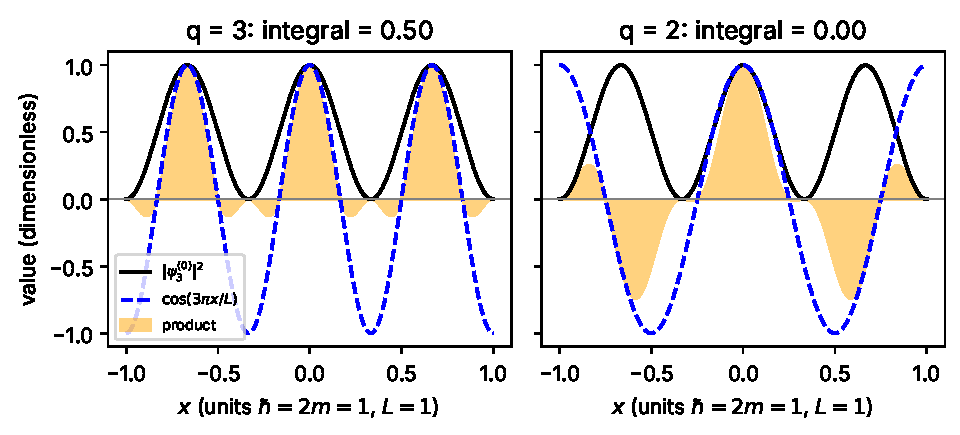
\includegraphics[width=0.85\linewidth]{figs/perturbation_overlap.pdf}
\caption{The first-order shift is an overlap integral. Both panels show the density $|\psi_3^{(0)}|^2$ of the third box state ($L=1$), a cosine perturbation, and their product (shaded). Left: $\cos(3\pi x/L)$ has the same ripple as the density, the product is mostly positive, and the integral is $1/2$. Right: $\cos(2\pi x/L)$ does not match, positive and negative areas cancel, and the integral is $0$, as \cref{eq:perturbation-boxcos} predicts.}
\label{fig:perturbation-overlap}
\end{figure}

\begin{sample}{One cosine in the running-example box}
Take the box of running example RE3, $L=44.883$, and add $\delta V=c\cos(3\pi x/L)$ with $c=10^{-3}$. Find the first-order shift of level 3, express it as a fraction of the spacing to level 4, and state what happens to levels 1, 2 and 4.

\textbf{Step 1: Unperturbed numbers.} $\pi/(2L)=\pi/89.766=0.0349976$, so $(\pi/2L)^2=1.22483\times10^{-3}$. Then $E_3^{(0)}=9(\pi/2L)^2=0.0110235$ and, by \cref{eq:perturbation-boxspacing}, $E_4^{(0)}-E_3^{(0)}=7(\pi/2L)^2=0.0085738$.

\textbf{Step 2: First-order shift.} By \cref{eq:perturbation-boxcos} with $q=n=3$ (odd), $\delta E_3^{(1)}=+c/2=5.0\times10^{-4}$.

\textbf{Step 3: Compare with the spacing.} $5.0\times10^{-4}/0.0085738=0.058$ of a spacing.

\textbf{Step 4: Other levels.} For $n\ne3$ the first-order shift is zero.

\[
\boxed{\delta E_3^{(1)}=5.0\times10^{-4}\approx0.058\ \text{spacings};\quad \delta E_{1,2,4}^{(1)}=0.}
\]
In \cref{sec:perturbation-second} we will find that the second-order correction to level 3 is $-2.83\times10^{-6}$, less than 1\% of the first-order shift; an exact computation (\cref{sec:perturbation-validity}) agrees with first plus second order to better than $10^{-7}$.
\end{sample}

\subsection{When parity kills the first order}

If the potential $V$ is even, $V(-x)=V(x)$, every state is either even or odd (Chapter~\ref{ch:bound-states}), so the density $|\psi_n^{(0)}(x)|^2$ is even in $x$. If $\delta V$ is odd, $\delta V(-x)=-\delta V(x)$, the integrand of \cref{eq:perturbation-first} is odd, and the integral over the symmetric interval $[-L,L]$ vanishes: the part from $[-L,0]$ cancels the part from $[0,L]$.

\begin{checkpoint}
A uniform force field adds $\delta V=Fx$ to the symmetric box (a ``tilt''). What are the first-order shifts of all levels?
\end{checkpoint}
\checkanswer{All zero. $|\psi_n^{(0)}|^2$ is even and $Fx$ is odd, so $\int|\psi_n^{(0)}|^2Fx\,\dd x=0$. The levels do move, but only at second order, as \cref{sec:perturbation-second} shows.}

\begin{keyideas}
\item First-order shift: $\delta E_n^{(1)}=\int|\psi_n^{(0)}|^2\delta V\,\dd x$, \cref{eq:perturbation-first}, a density-weighted average of $\delta V$.
\item A constant $\delta V=c$ shifts every level by exactly $c$.
\item In the box, $\cos(q\pi x/L)$ shifts only level $q$ at first order, by $(-1)^{q+1}c/2$, \cref{eq:perturbation-boxcos}.
\item In an even potential, an odd $\delta V$ gives zero first-order shift for every level.
\end{keyideas}

%======================================================================
\section{The sensitivity matrix and linearization}\label{sec:perturbation-sensitivity}

\subsection{Many basis functions at once}

In the paper the correction is not one cosine but a sum,
\begin{equation}
\delta V(x)=\sum_{k=0}^{M-1}c_k\,\phi_k(x),
\label{eq:perturbation-basis}
\end{equation}
where the $\phi_k$ are fixed \emph{basis functions} (by default $\phi_k=\cos(k\pi x/L)$), $M$ is the number of them, and the real numbers $c_k$ are the coefficients we may adjust. The first-order shift \cref{eq:perturbation-first} is linear in $\delta V$: the integral of a sum is the sum of the integrals. Hence
\begin{align}
\delta E_n^{(1)}&=\int_{-L}^{L}|\psi_n^{(0)}|^2\sum_{k=0}^{M-1}c_k\phi_k\,\dd x
=\sum_{k=0}^{M-1}\left(\int_{-L}^{L}|\psi_n^{(0)}|^2\phi_k\,\dd x\right)c_k \notag\\
&=\sum_{k=0}^{M-1}A_{nk}\,c_k,
\label{eq:perturbation-linear}
\end{align}
with the \emph{sensitivity matrix}
\begin{equation}
A_{nk}=\int_{-L}^{L}|\psi_n(x)|^2\,\phi_k(x)\,\dd x .
\label{eq:perturbation-Ank}
\end{equation}
Row $n$ of $A$ tells you how level $n$ responds to each basis function; column $k$ tells you how basis function $k$ moves every level. If we collect the shifts into a vector $\delta\bm E$ and the coefficients into a vector $\bm c$ (Chapter~\ref{ch:linear-algebra}), \cref{eq:perturbation-linear} is the matrix equation $\delta\bm E\approx A\bm c$. Replacing the true, complicated dependence of the levels on $\bm c$ by this linear one is called \emph{linearization}. Its error is of second order in $\bm c$, the subject of the next section.

Two facts hold for any normalized state:
\begin{itemize}
\item The constant basis function $\phi_0=1$ has $A_{n0}=\int|\psi_n|^2\dd x=1$ for every $n$: column 0 of $A$ is all ones.
\item For the box with cosines, \cref{eq:perturbation-boxcos} gives
\begin{equation}
A_{nk}^{\text{box}}=\delta_{k0}+\frac{(-1)^{k+1}}{2}\,\delta_{nk}\qquad(k\ge0,\ n\ge1),
\label{eq:perturbation-Abox}
\end{equation}
a column of ones plus a diagonal of $\pm\tfrac12$.
\end{itemize}

\begin{checkpoint}
In the box with the $M=10$ cosines $k=0,\dots,9$, which levels can be moved \emph{individually} at first order, and how does level 50 respond?
\end{checkpoint}
\checkanswer{Levels 1 to 9: level $n\le9$ is the only level that responds to $c_n$. Level 50 responds only to $c_0$, which moves all levels together, so at first order $\delta E_{50}=c_0$.}

\subsection{A first look at ``memorizing''}

\begin{sample}{Tuning three box levels with three cosines}
Box with $L=1$; basis $\phi_0=1$, $\phi_1=\cos(\pi x/L)$, $\phi_2=\cos(2\pi x/L)$. Find $c_0,c_1,c_2$ such that, at first order, levels 1, 2, 3 shift by $0.01$, $-0.02$ and $0.005$. Then predict, at first order, the shift of level 4.

\textbf{Step 1: The sensitivity matrix.} By \cref{eq:perturbation-Abox}, with rows $n=1,2,3$ and columns $k=0,1,2$:
\[
A=\begin{pmatrix}1&\tfrac12&0\\[2pt]1&0&-\tfrac12\\[2pt]1&0&0\end{pmatrix}.
\]

\textbf{Step 2: Write the equations.} $A\bm c=\delta\bm E$ reads
\[
c_0+\tfrac12c_1=0.01,\qquad c_0-\tfrac12c_2=-0.02,\qquad c_0=0.005 .
\]

\textbf{Step 3: Solve.} The third equation gives $c_0=0.005$. Then $c_1=2(0.01-0.005)=0.01$ and $c_2=-2(-0.02-0.005)=0.05$.

\textbf{Step 4: Predict level 4.} Row 4 of $A^{\text{box}}$ is $(1,0,0)$, so $\delta E_4^{(1)}=c_0=0.005$, and the same holds for every $n\ge3$.

\[
\boxed{c_0=0.005,\ c_1=0.01,\ c_2=0.05;\qquad \delta E_4^{(1)}=0.005.}
\]
An exact computation (\cref{sec:perturbation-validity}) confirms the shifts of levels 1 to 4 to within $10^{-4}$. Notice what the fit has learned about level 4: nothing that came from levels 1 and 2. Whatever pattern you ask levels 1 to 3 to follow, level 4 receives only the common offset $c_0$. The coefficients reproduce the three targets perfectly and carry no information about the next level. This is the simplest possible picture of a model that memorizes its training data; Chapter~\ref{ch:generalization} develops the idea in general.
\end{sample}

\subsection{The sensitivity matrix is the exact derivative}

Equation~\eqref{eq:perturbation-linear} is a statement about small $\bm c$ near $\bm c=0$. But nothing in the derivation required the unperturbed problem to be the box. Suppose we are at some coefficient vector $\bm c$, with Hamiltonian $H(\bm c)=H_0+\sum_kc_k\phi_k$, levels $E_n(\bm c)$ and normalized states $\psi_n(\bm c)$. Increase one coefficient, $c_k\to c_k+\eta$. Relative to $H(\bm c)$ this is a perturbation $\eta\phi_k$, and \cref{eq:perturbation-first}, applied with $H(\bm c)$ as the ``unperturbed'' Hamiltonian, gives
\[
E_n(\bm c+\eta\,\hat{\bm e}_k)=E_n(\bm c)+\eta\int|\psi_n(\bm c)|^2\phi_k\,\dd x+\order(\eta^2),
\]
where $\hat{\bm e}_k$ is the vector with 1 in place $k$ and zeros elsewhere. Subtract $E_n(\bm c)$, divide by $\eta$, and let $\eta\to0$:
\begin{equation}
\frac{\partial E_n}{\partial c_k}\bigg|_{\bm c}=\int_{-L}^{L}|\psi_n(\bm c)|^2\,\phi_k\,\dd x=A_{nk}(\bm c).
\label{eq:perturbation-HF}
\end{equation}
This is the \emph{Hellmann--Feynman theorem}: the derivative of an eigenvalue with respect to a parameter in the Hamiltonian is the expectation value of the derivative of the Hamiltonian. (Problem~9 asks you to derive it directly, without perturbation theory.) The symbol $\partial/\partial c_k$ is a partial derivative: the rate of change with respect to $c_k$ with all other coefficients held fixed. The matrix $A_{nk}(\bm c)$ evaluated with the \emph{current} wavefunctions is therefore not an approximation at all: it is the exact Jacobian (matrix of first derivatives) of the levels with respect to the coefficients. This is why it is the natural tool for fitting, \cref{sec:perturbation-fitting}.

\subsection{Computing $A$ on a grid}

On a computer, wavefunctions are represented by their values $\psi_n(x_j)$ on grid points $x_j$ with spacing $h$ (Chapter~\ref{ch:eigen}; full details in Chapter~\ref{ch:finite-differences}). Integrals become sums, $\int f\,\dd x\approx\sum_jf(x_j)h$. The following listing builds the finite-difference Hamiltonian, finds the first 100 eigenpairs with \texttt{eigh\_tridiagonal}, and forms $A$ as one matrix product.

\begin{pycode}
import numpy as np
from scipy.linalg import eigh_tridiagonal

L, N, nlev, M = 44.883, 3000, 100, 100
h = 2 * L / (N + 1)                       # grid spacing
x = -L + h * np.arange(1, N + 1)          # interior grid points
V = np.zeros(N)                           # the box; put any V(x) here
d = 2 / h**2 + V                          # diagonal
e = -np.ones(N - 1) / h**2                # off-diagonal
E, psi = eigh_tridiagonal(d, e, select='i',
                          select_range=(0, nlev - 1))
psi = psi / np.sqrt(h)                    # now sum(psi**2) * h = 1
k = np.arange(M)
phi = np.cos(np.outer(x, k) * np.pi / L)  # phi[j, k] = cos(k pi x_j / L)
A = (psi**2 * h).T @ phi                  # A[n-1, k]
print(A[0, 0], A[2, 3], A[2, 2])          # about 1, 0.5 and 0
\end{pycode}

\begin{pitfall}
\texttt{eigh\_tridiagonal} returns eigenvectors normalized so that $\sum_j\psi_j^2=1$, the normalization of a vector. A wavefunction needs $\sum_j\psi_j^2h=1$, the discrete version of $\int|\psi|^2\dd x=1$. Forgetting the division by $\sqrt h$ multiplies every $A_{nk}$ by $h$, so the constant column is $h$ instead of 1 and every predicted shift is wrong by a factor $1/h$. The paper states this normalization explicitly (App.~A, step 9: ``$\psi$ normalized $\sum\psi^2dx=1$'').
\end{pitfall}

\Cref{fig:perturbation-sensitivity} compares the sensitivity matrix of the box with that of the Wu--Sprung potential. That potential (defined by the paper's Eq.~(2) and derived in Chapter~\ref{ch:wu-sprung}) is even, has its minimum $V_0=3.10073\pi$ at $x=0$, and rises to $V=1000$ at $x=\pm44.883$. All you need here is that its low levels are confined to a central region much narrower than the box: level 20, near $E\approx77$, turns at $|x|\approx5.4$, less than an eighth of $L$. Over that region $\cos(k\pi x/L)\approx1$ for the first few $k$, so those columns behave almost like the constant column for low levels: for example $A_{20,1}>0.9$. The clean diagonal of the box is gone; level 20 has sizeable sensitivity (above 0.1) to at least five different cosines with $k\ge1$, and each cosine moves many levels.

\begin{figure}[htbp]\centering
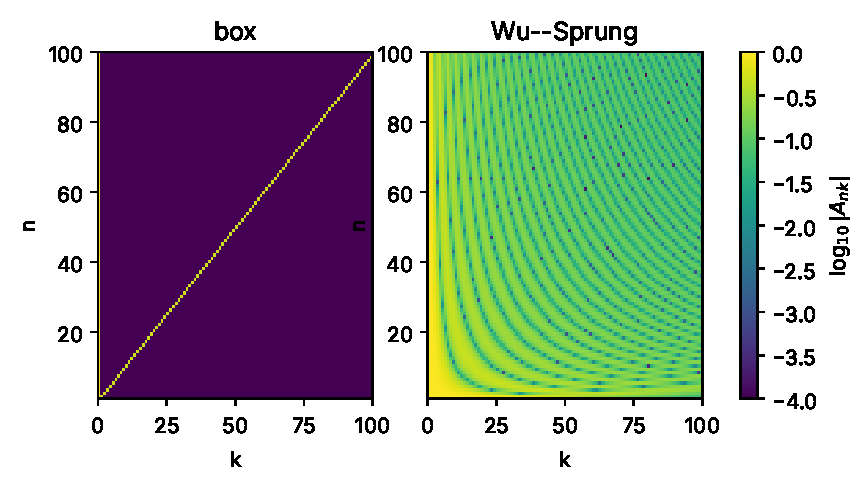
\includegraphics[width=0.95\linewidth]{figs/perturbation_sensitivity.pdf}
\caption{Magnitude $|A_{nk}|$ of the first-order sensitivity matrix, \cref{eq:perturbation-Ank}, for cosine basis functions $\cos(k\pi x/L)$, $L=44.883$, levels $n=1$--$100$, computed on a 3000-point finite-difference grid (logarithmic color scale). Left: the box, where $A$ is a column of ones ($k=0$) plus a diagonal of magnitude $1/2$, \cref{eq:perturbation-Abox}. Right: the Wu--Sprung potential, where each level responds to a broad band of cosines and low cosines act almost like the constant mode for low levels.}
\label{fig:perturbation-sensitivity}
\end{figure}

\begin{keyideas}
\item For $\delta V=\sum_kc_k\phi_k$, the first-order shifts are linear in $\bm c$: $\delta\bm E\approx A\bm c$, with $A_{nk}=\int|\psi_n|^2\phi_k\,\dd x$, \cref{eq:perturbation-linear,eq:perturbation-Ank}.
\item $A_{n0}=1$ for the constant mode; in the box with cosines, $A$ is otherwise diagonal.
\item Evaluated with the current wavefunctions, $A_{nk}$ is the exact derivative $\partial E_n/\partial c_k$ (Hellmann--Feynman, \cref{eq:perturbation-HF}).
\item On a grid, $A=(\psi^2h)^{\top}\phi$ with $\sum_j\psi_j^2h=1$.
\end{keyideas}

%======================================================================
\section{Second order and level repulsion}\label{sec:perturbation-second}

\subsection{The first-order wavefunction}

Return to \cref{eq:perturbation-projected1} with $k\ne n$. Then $\delta_{kn}=0$ and
\begin{equation}
a_k=\frac{W_{kn}}{E_n^{(0)}-E_k^{(0)}}\qquad(k\ne n).
\label{eq:perturbation-ak-result}
\end{equation}
(We divided by $E_k^{(0)}-E_n^{(0)}$ and moved the minus sign into the denominator.) This determines every coefficient of $\psi_n^{(1)}$ except $a_n$. To fix $a_n$, use the freedom in normalization: any constant multiple of an eigenfunction is still an eigenfunction, so we may choose the scale of $\psi_n$ by requiring $\int\psi_n^{(0)*}\psi_n\,\dd x=1$ exactly, for all $\varepsilon$. Inserting the series, this says $1+\varepsilon a_n+\order(\varepsilon^2)=1$, so $a_n=0$ (and likewise the overlap of $\psi_n^{(0)}$ with $\psi_n^{(2)}$ vanishes). This choice, called intermediate normalization, does not affect any energy: the energies are fixed by the eigenvalue equation, not by the scale of $\psi_n$. If a normalized wavefunction is needed, we rescale at the end. Hence, by \cref{eq:perturbation-expand},
\begin{equation}
\psi_n^{(1)}=\sum_{k\ne n}\frac{W_{kn}}{E_n^{(0)}-E_k^{(0)}}\,\psi_k^{(0)} .
\label{eq:perturbation-psi1}
\end{equation}
The perturbation mixes a little of every other state into state $n$; the amount is large when the coupling $W_{kn}$ is large and when the two levels are close.

\subsection{Derivation of the second-order shift}

Multiply the order-$\varepsilon^2$ equation \cref{eq:perturbation-order2} by $\psi_n^{(0)*}$ and integrate. The left side is $(E_n^{(0)}-E_n^{(0)})\int\psi_n^{(0)*}\psi_n^{(2)}\dd x=0$, by exactly the Hermiticity argument used for \cref{eq:perturbation-projected1} with $k=n$. The right side gives three terms:
\begin{align*}
0&=E_n^{(1)}\int\psi_n^{(0)*}\psi_n^{(1)}\dd x-\int\psi_n^{(0)*}W\psi_n^{(1)}\dd x+E_n^{(2)}\int\psi_n^{(0)*}\psi_n^{(0)}\dd x\\
&=E_n^{(1)}a_n-\int\psi_n^{(0)*}W\psi_n^{(1)}\dd x+E_n^{(2)}
\quad\text{(by \cref{eq:perturbation-ak,eq:perturbation-orthonormal})}\\
&=-\int\psi_n^{(0)*}W\psi_n^{(1)}\dd x+E_n^{(2)}
\quad\text{($a_n=0$)}.
\end{align*}
So $E_n^{(2)}=\int\psi_n^{(0)*}W\psi_n^{(1)}\dd x$. Substitute \cref{eq:perturbation-psi1} and exchange the sum and the integral (each term is a finite integral; for an infinite sum this exchange is part of the trust placed in the power-series assumption):
\begin{equation}
E_n^{(2)}=\sum_{k\ne n}\frac{W_{kn}}{E_n^{(0)}-E_k^{(0)}}\int\psi_n^{(0)*}W\psi_k^{(0)}\dd x
=\sum_{k\ne n}\frac{W_{nk}\,W_{kn}}{E_n^{(0)}-E_k^{(0)}} .
\label{eq:perturbation-second-general}
\end{equation}
This general form needs only $H_0$ to be Hermitian. If $W$ is also real, \cref{eq:perturbation-hermmat} gives $W_{nk}=W_{kn}^*$, so $W_{nk}W_{kn}=|W_{kn}|^2$. Restoring $\delta V=\varepsilon W$ and writing $\delta V_{nm}=\varepsilon W_{nm}=\bra{n}\delta V\ket{m}$ (many books write simply $V_{nm}$), the energy through second order is
\begin{equation}
\boxed{E_n\approx E_n^{(0)}+\delta V_{nn}+\sum_{m\ne n}\frac{|\delta V_{nm}|^2}{E_n^{(0)}-E_m^{(0)}}} .
\label{eq:perturbation-second}
\end{equation}

\begin{pitfall}
Watch the order in the denominator: it is $E_n^{(0)}-E_m^{(0)}$, the level you are computing minus the other level. Reversing it flips the sign of every term. And the term $m=n$ is excluded; including it would divide by zero.
\end{pitfall}

\subsection{Level repulsion}

Each term of the sum in \cref{eq:perturbation-second} has a positive numerator. Its sign is the sign of the denominator:
\begin{itemize}
\item a level $m$ \emph{above} $n$ ($E_m^{(0)}>E_n^{(0)}$) contributes a negative term: it pushes level $n$ down;
\item a level $m$ \emph{below} $n$ contributes a positive term: it pushes level $n$ up.
\end{itemize}
Coupled levels push each other apart, and close levels push hardest. This is \emph{level repulsion}. Its statistical consequences for large spectra, including the Riemann zeros, are the subject of Chapter~\ref{ch:level-statistics}.

\begin{checkpoint}
What is the sign of the second-order shift of the ground state $n=1$, whatever the (real) perturbation?
\end{checkpoint}
\checkanswer{Negative or zero. Every other level lies above the ground state, so every denominator $E_1^{(0)}-E_m^{(0)}$ is negative while every numerator $|\delta V_{1m}|^2$ is non-negative.}

The cleanest way to see repulsion is the two-level system, which we can solve exactly. Recall from Chapter~\ref{ch:eigen} the eigenvalues of a $2\times2$ Hermitian matrix:
\[
H=\begin{pmatrix}E_1&v\\ v^*&E_2\end{pmatrix},\qquad E_1<E_2 .
\]
The characteristic equation $\det(H-\lambda I)=0$ is $(E_1-\lambda)(E_2-\lambda)-|v|^2=0$, that is
\[
\lambda^2-(E_1+E_2)\lambda+E_1E_2-|v|^2=0 .
\]
By the quadratic formula,
\begin{align}
\lambda_\pm&=\frac{E_1+E_2}{2}\pm\sqrt{\frac{(E_1+E_2)^2}{4}-E_1E_2+|v|^2}
=\frac{E_1+E_2}{2}\pm\sqrt{\Delta^2+|v|^2},
\label{eq:perturbation-twolevel}
\end{align}
where $\Delta=(E_2-E_1)/2>0$ and we used $\tfrac14(E_1+E_2)^2-E_1E_2=\tfrac14(E_2-E_1)^2$. When $|v|\ll\Delta$, write $\sqrt{\Delta^2+|v|^2}=\Delta\sqrt{1+y}$ with $y=|v|^2/\Delta^2\ll1$ and use $\sqrt{1+y}\approx1+y/2$ (Chapter~\ref{ch:asymptotics}; the neglected term is of order $y^2$):
\[
\sqrt{\Delta^2+|v|^2}\approx\Delta+\frac{|v|^2}{2\Delta}=\frac{E_2-E_1}{2}+\frac{|v|^2}{E_2-E_1}.
\]
Then
\[
\lambda_-\approx E_1-\frac{|v|^2}{E_2-E_1},\qquad\lambda_+\approx E_2+\frac{|v|^2}{E_2-E_1},
\]
which is exactly \cref{eq:perturbation-second} for two levels (the diagonal of the perturbation is zero here; $\delta V_{12}=v$). The exact formula shows something the expansion does not: as you vary the diagonal energies so that the two levels approach each other, the gap $\lambda_+-\lambda_-=2\sqrt{\Delta^2+|v|^2}$ never falls below $2|v|$. The levels \emph{avoid crossing} (\cref{fig:perturbation-repulsion}).

\begin{figure}[htbp]\centering
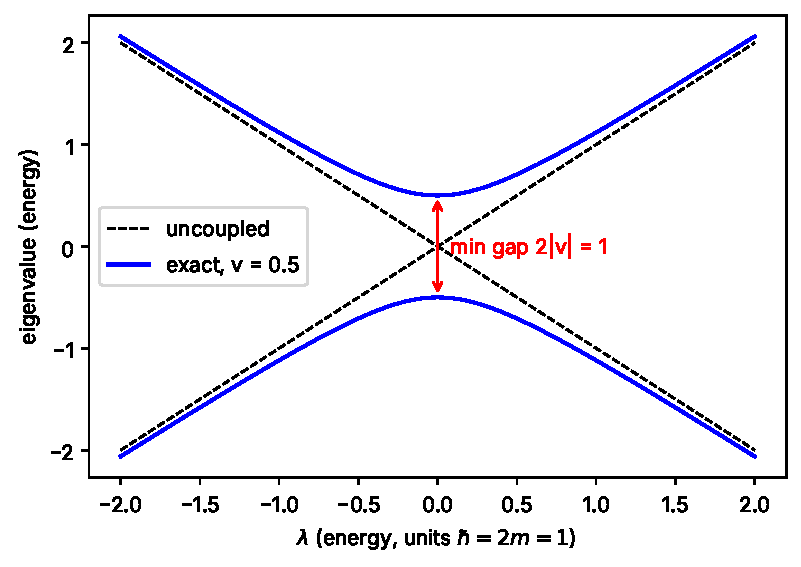
\includegraphics[width=0.85\linewidth]{figs/perturbation_repulsion.pdf}
\caption{Level repulsion in the two-level system $H=\begin{pmatrix}\lambda&v\\v&-\lambda\end{pmatrix}$. Dashed: the uncoupled levels $\pm\lambda$, which cross at $\lambda=0$. Solid: the exact eigenvalues $\pm\sqrt{\lambda^2+v^2}$ for $v=0.5$, which avoid crossing with minimum gap $2|v|=1$. Far from the crossing the coupled levels approach the uncoupled ones, pushed apart by $v^2/(2|\lambda|)$ each, as second-order perturbation theory predicts.}
\label{fig:perturbation-repulsion}
\end{figure}

\begin{sample}{Two levels, exact and perturbative}
Take $E_1=1$, $E_2=3$, $v=0.5$. Compute the exact eigenvalues and the second-order estimates.

\textbf{Step 1: Exact.} $\Delta=(3-1)/2=1$, so by \cref{eq:perturbation-twolevel} $\lambda_\pm=2\pm\sqrt{1+0.25}=2\pm1.118034$, that is $0.881966$ and $3.118034$.

\textbf{Step 2: Second order.} $|v|^2/(E_2-E_1)=0.25/2=0.125$, so $\lambda_-\approx1-0.125=0.875$ and $\lambda_+\approx3+0.125=3.125$.

\textbf{Step 3: Compare.} The errors are $0.0070$, about 6\% of the shift. Here $|v|/\Delta=0.5$ is not very small, and the neglected term in $\sqrt{1+y}$ (of relative size $y/4=1/16$) is visible.

\[
\boxed{\text{exact }0.881966,\ 3.118034;\qquad\text{second order }0.875,\ 3.125.}
\]
\end{sample}

\subsection{The box with a tilt}

To do the tilt we need the matrix elements $x_{nm}=\int\psi_n^{(0)}x\,\psi_m^{(0)}\dd x$ of the box. With $u=x+L$ and $a=2L$, $\psi_n^{(0)}=\sqrt{2/a}\,\sin(n\pi u/a)$ and $x=u-L$, so
\[
x_{nm}=\frac2a\int_0^a u\,\sin\frac{n\pi u}{a}\sin\frac{m\pi u}{a}\,\dd u-L\,\delta_{nm}.
\]
We need one integral, for a nonzero integer $j$; integrating by parts with $U=u$ and $\dd V=\cos(j\pi u/a)\dd u$:
\begin{align}
\int_0^a u\cos\frac{j\pi u}{a}\dd u
&=\Bigl[u\,\frac{a}{j\pi}\sin\frac{j\pi u}{a}\Bigr]_0^a-\frac{a}{j\pi}\int_0^a\sin\frac{j\pi u}{a}\dd u \notag\\
&=0+\frac{a}{j\pi}\Bigl[\frac{a}{j\pi}\cos\frac{j\pi u}{a}\Bigr]_0^a
=\Bigl(\frac{a}{j\pi}\Bigr)^2\bigl[(-1)^j-1\bigr].
\label{eq:perturbation-ucos}
\end{align}
Now let $n\ne m$ and use $\sin A\sin B=\tfrac12[\cos(A-B)-\cos(A+B)]$:
\[
x_{nm}=\frac1a\left[\Bigl(\frac{a}{(n-m)\pi}\Bigr)^2\bigl((-1)^{n-m}-1\bigr)-\Bigl(\frac{a}{(n+m)\pi}\Bigr)^2\bigl((-1)^{n+m}-1\bigr)\right].
\]
Since $n-m$ and $n+m$ differ by the even number $2m$, $(-1)^{n-m}=(-1)^{n+m}$. If $n+m$ is even both brackets vanish and $x_{nm}=0$. If $n+m$ is odd both brackets equal $-2$, and
\[
x_{nm}=-\frac{2a}{\pi^2}\left[\frac{1}{(n-m)^2}-\frac{1}{(n+m)^2}\right]=-\frac{2a}{\pi^2}\,\frac{4nm}{(n^2-m^2)^2},
\]
because $(n+m)^2-(n-m)^2=4nm$ and $(n-m)^2(n+m)^2=(n^2-m^2)^2$. With $a=2L$:
\begin{equation}
x_{nm}=\begin{cases}-\dfrac{16Lnm}{\pi^2(n^2-m^2)^2}, & n+m\ \text{odd},\\[8pt] 0, & n+m\ \text{even}.\end{cases}
\label{eq:perturbation-xnm}
\end{equation}
The diagonal $x_{nn}$ vanishes by parity (\cref{sec:perturbation-first}). States of the same parity are not coupled by the odd function $x$; states of opposite parity are.

\begin{sample}{The quadratic shift of a tilted box}
Box with $L=1$, $\delta V=Fx$ with $F=1$. Find the second-order shift of the ground state and compare with an exact computation.

\textbf{Step 1: Which states couple.} By \cref{eq:perturbation-xnm}, $n=1$ couples only to even $m$: $x_{1m}=-16m/[\pi^2(m^2-1)^2]$. For $m=2$, $x_{12}=-32/(9\pi^2)=-0.36025$.

\textbf{Step 2: Denominators.} $E_1^{(0)}-E_m^{(0)}=(\pi/2L)^2(1-m^2)=-\tfrac{\pi^2}{4}(m^2-1)$ for $L=1$.

\textbf{Step 3: Assemble.} By \cref{eq:perturbation-second},
\[
E_1^{(2)}=F^2\sum_{m\ \text{even}}\frac{x_{1m}^2}{E_1^{(0)}-E_m^{(0)}}
=-F^2\sum_{m\ \text{even}}\frac{256m^2}{\pi^4(m^2-1)^4}\cdot\frac{4}{\pi^2(m^2-1)}
=-F^2\frac{1024}{\pi^6}\,S,
\]
with $S=\sum_{m=2,4,6,\dots}m^2/(m^2-1)^5$. The terms fall off fast: $m=2$ gives $4/243=0.016461$, $m=4$ gives $2.1\times10^{-5}$, and the full sum is $S=0.016483$. (It equals $(15-\pi^2)\pi^2/3072$, a closed form we check numerically but do not derive.) Since $1024/\pi^6=1.06513$, $E_1^{(2)}=-0.017556\,F^2$.

\textbf{Step 4: Compare.} First order predicts no change. Second order predicts $E_1\approx2.467401-0.017556=2.449845$. Exact diagonalization (the method of \cref{sec:perturbation-validity}) gives $2.44987$: the two differ by only about $2\times10^{-5}$.

\[
\boxed{E_1^{(2)}=-0.017556\,F^2\ \ (L=1);\qquad E_1(F{=}1)\approx2.44987\ \text{exactly}.}
\]
The ground state moves down, as every ground state must at second order, and quadratically in $F$ (the shift does not care which way the box is tilted). In atomic physics the analogous effect is the quadratic Stark effect.
\end{sample}

\subsection{The box with a cosine, at second order}

For $\delta V=c\cos(q\pi x/L)$ we also need off-diagonal elements. With $\theta=\pi u/2L$ (which runs from 0 to $\pi$ as $u$ runs over the box), $\psi_n^{(0)}\psi_m^{(0)}=\tfrac1L\sin n\theta\sin m\theta=\tfrac{1}{2L}[\cos(n-m)\theta-\cos(n+m)\theta]$ and $\cos(q\pi x/L)=(-1)^q\cos2q\theta$. Using $\dd u=(2L/\pi)\dd\theta$ and $\int_0^\pi\cos j\theta\cos l\theta\,\dd\theta=\tfrac\pi2\delta_{jl}$ for positive integers $j,l$ (and $0$ if one of them is $0$ and the other is not; both facts follow from the product-to-sum formula as in \cref{eq:perturbation-cosint}),
\begin{equation}
\bra{n}\cos\tfrac{q\pi x}{L}\ket{m}=\frac{(-1)^q}{2}\Bigl[\delta_{|n-m|,2q}-\delta_{n+m,2q}\Bigr]\qquad(q\ge1).
\label{eq:perturbation-cosmat}
\end{equation}
So the cosine with index $q$ couples level $n$ to the levels $n\pm2q$ (with $+\tfrac12(-1)^q$) and to the level $2q-n$ (with $-\tfrac12(-1)^q$). Setting $m=n$ recovers \cref{eq:perturbation-boxcos}: only $n=q$ has a diagonal element.

\begin{sample}{Ground state with $\cos(\pi x/L)$}
Box with $L=1$, $\delta V=c\cos(\pi x/L)$, $c=1$. Compute the ground-state energy at first and second order, and compare with the exact value.

\textbf{Step 1: Matrix elements.} With $q=1$, \cref{eq:perturbation-cosmat}: $\delta V_{11}=-\tfrac12(-1)c=c/2$ (from $n+m=2$), and $\delta V_{13}=\tfrac12(-1)c=-c/2$ (from $|n-m|=2$). No other $m$ couples to $n=1$.

\textbf{Step 2: First order.} $E_1\approx\pi^2/4+c/2=2.467401+0.5=2.967401$.

\textbf{Step 3: Second order.} $E_1^{(0)}-E_3^{(0)}=\tfrac{\pi^2}{4}(1-9)=-2\pi^2$, so the shift is $(c^2/4)/(-2\pi^2)=-c^2/(8\pi^2)=-0.012665$ (for general $L$, $-c^2L^2/8\pi^2$). Thus $E_1\approx2.954736$.

\textbf{Step 4: Exact.} Exact diagonalization gives $E_1=2.954413$.

\[
\boxed{\text{first order }2.967401,\quad\text{second order }2.954736,\quad\text{exact }2.954413.}
\]
The first-order error is $1.3\times10^{-2}$, the second-order error $3.2\times10^{-4}$. Most of the remainder has a simple origin: the first-order shift $+c/2$ moved level 1 up, closer to level 3, so the true denominator is nearer to $E_1^{(0)}+c/2-E_3^{(0)}$. Using that denominator gives $2.954407$, within $10^{-5}$ of the exact value. (Systematically, this is part of the third-order correction, which we do not derive.)
\end{sample}

Returning to the RE3 box sample: for $q=n=3$, \cref{eq:perturbation-cosmat} couples level 3 to level 9 with $\delta V_{39}=-c/2$, and $E_3^{(0)}-E_9^{(0)}=(\pi/2L)^2(9-81)=-0.088188$, so the second-order shift is $(c/2)^2/(-0.088188)=-2.83\times10^{-6}$ for $c=10^{-3}$, as promised.

\begin{keyideas}
\item First-order wavefunction: $\psi_n^{(1)}=\sum_{k\ne n}W_{kn}\psi_k^{(0)}/(E_n^{(0)}-E_k^{(0)})$, \cref{eq:perturbation-psi1}.
\item Second-order shift: $\sum_{m\ne n}\delta V_{nm}\delta V_{mn}/(E_n^{(0)}-E_m^{(0)})$, which equals $\sum_{m\ne n}|\delta V_{nm}|^2/(E_n^{(0)}-E_m^{(0)})$ for real $\delta V$, \cref{eq:perturbation-second-general,eq:perturbation-second}.
\item Levels above push down, levels below push up: level repulsion; the ground state always moves down at second order.
\item Box matrix elements: $x_{nm}$ in \cref{eq:perturbation-xnm}, cosines in \cref{eq:perturbation-cosmat}.
\end{keyideas}

%======================================================================
\section{Exact diagonalization and the validity condition}\label{sec:perturbation-validity}

\subsection{The matrix method}

How did we get the ``exact'' numbers above? Expand the unknown eigenfunction of $H=H_0+\delta V$ in the unperturbed states, $\psi=\sum_ma_m\psi_m^{(0)}$ (\cref{eq:perturbation-expand}). Insert into $H\psi=E\psi$:
\[
\sum_ma_m\bigl(E_m^{(0)}+\delta V\bigr)\psi_m^{(0)}=E\sum_ma_m\psi_m^{(0)} .
\]
Multiply by $\psi_k^{(0)*}$ and integrate; by \cref{eq:perturbation-orthonormal,eq:perturbation-matel},
\begin{equation}
\sum_m\Bigl(E_m^{(0)}\delta_{km}+\delta V_{km}\Bigr)a_m=E\,a_k\qquad\text{for every }k.
\label{eq:perturbation-galerkin}
\end{equation}
This is a matrix eigenvalue problem (Chapter~\ref{ch:eigen}) for the matrix $H_{km}=E_k^{(0)}\delta_{km}+\delta V_{km}$, the unperturbed energies on the diagonal plus the matrix of the perturbation. It is exact but infinite. We keep the first $N_b$ states and diagonalize the $N_b\times N_b$ matrix; then we repeat with a larger $N_b$ and accept the answer when it no longer changes. Truncation works well here because a state far above level $n$ couples to it through a large denominator. This approach is often called the Galerkin or Rayleigh--Ritz method. For the box with cosines we know every matrix element in closed form, \cref{eq:perturbation-cosmat}, so the method is easy:

\begin{pycode}
import numpy as np
L, Nb = 1.0, 60                     # box half-width, number of sine states
n = np.arange(1, Nb + 1)
E0 = (n * np.pi / (2 * L))**2       # unperturbed levels
D = np.abs(n[:, None] - n[None, :]) # |n - m|
S = n[:, None] + n[None, :]         # n + m

def cos_matrix(q):
    """<n|cos(q pi x / L)|m> for q >= 1, Eq. (cosmat)."""
    return 0.5 * (-1)**q * ((D == 2*q) * 1.0 - (S == 2*q) * 1.0)

c = 1.0
H = np.diag(E0) + c * cos_matrix(1)
E = np.linalg.eigvalsh(H)           # exact levels, sorted
first  = E0[0] + c / 2
second = first - c**2 * L**2 / (8 * np.pi**2)
print(E[0], first, second)          # 2.954413  2.967401  2.954736
\end{pycode}

With $N_b=60$ the ground-state energy agrees with $N_b=200$ to many digits; the CHECKS script for this chapter also confirms it independently with a finite-difference grid (the method of Chapter~\ref{ch:finite-differences}).

\begin{checkpoint}
Why does the matrix of \cref{eq:perturbation-galerkin} come out real and symmetric for the box with a real $\delta V$, and why does that matter for the solver?
\end{checkpoint}
\checkanswer{The unperturbed states are real and $\delta V$ is real, so $\delta V_{km}=\delta V_{mk}$ is real (\cref{eq:perturbation-hermmat}); the diagonal $E_k^{(0)}$ is real. A real symmetric matrix has real eigenvalues and orthogonal eigenvectors (Chapter~\ref{ch:eigen}), so we can use the fast, stable symmetric solver \texttt{eigvalsh}.}

\subsection{When does perturbation theory work?}

\Cref{fig:perturbation-validity} plots the ground-state energy of the $L=1$ box with $\delta V=c\cos(\pi x/L)$ as $c$ grows. For small $c$ the three curves agree; second order hugs the exact curve much longer than first order; and eventually both depart.

\begin{figure}[htbp]\centering
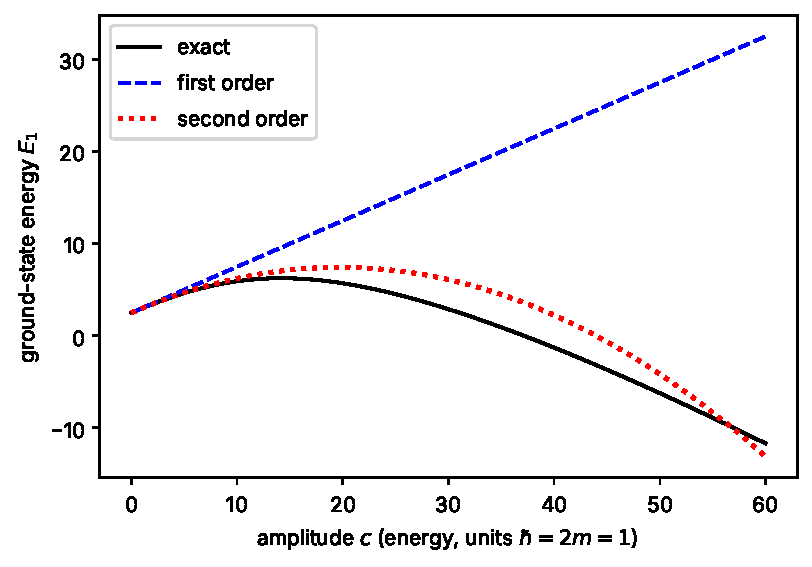
\includegraphics[width=0.85\linewidth]{figs/perturbation_validity.pdf}
\caption{Ground-state energy of the box ($L=1$) with $\delta V=c\cos(\pi x/L)$, as a function of the amplitude $c$. Solid: exact diagonalization, \cref{eq:perturbation-galerkin}. Dashed: first order, $E_1^{(0)}+c/2$. Dotted: second order, $E_1^{(0)}+c/2-c^2/8\pi^2$. The coupled level is $E_3^{(0)}$, at a distance $2\pi^2\approx19.7$; perturbation theory is accurate while the coupling $c/2$ is small compared with that distance and degrades as $c/2$ approaches it.}
\label{fig:perturbation-validity}
\end{figure}

Where does the expansion break down? Look at the first-order wavefunction \cref{eq:perturbation-psi1}: it mixes state $k$ into state $n$ with amplitude $\delta V_{kn}/(E_n^{(0)}-E_k^{(0)})$. The whole expansion assumes the perturbed state is \emph{mostly} the unperturbed one, so these amplitudes must be small. The same ratio controls how big the second-order term is compared with the first-order term. This gives the practical \emph{validity condition}:
\begin{equation}
\bigl|\delta V_{nm}\bigr|\ll\bigl|E_n^{(0)}-E_m^{(0)}\bigr|\qquad\text{for all }m\ne n,\ \text{in particular for the nearest coupled levels}.
\label{eq:perturbation-validity}
\end{equation}
Status: this is a heuristic rule of thumb, not a theorem with a sharp threshold; whether and how fast the full series converges is a harder question (see the box in \cref{sec:perturbation-tools}). The previous sample adds one refinement: diagonal shifts $\delta V_{nn}$ that are comparable to spacings change the effective gaps, so they should be small too. In words: \emph{the perturbation must be small compared with the spacing between the levels it couples}.

\begin{sample}{How large may the cosine be?}
For the box and $\delta V=c\cos(\pi x/L)$, estimate the largest $c$ for which perturbation theory is reliable for level $n\ge3$, and for $n=1$.

\textbf{Step 1: Couplings.} By \cref{eq:perturbation-cosmat} with $q=1$, level $n\ge3$ couples to $n-2$ and $n+2$ with $|\delta V|=c/2$ (the partner $2-n$ does not exist).

\textbf{Step 2: Nearest coupled distance.} $E_n^{(0)}-E_{n-2}^{(0)}=(\pi/2L)^2[n^2-(n-2)^2]=4(n-1)(\pi/2L)^2$, smaller than $E_{n+2}^{(0)}-E_n^{(0)}=4(n+1)(\pi/2L)^2$.

\textbf{Step 3: Apply \cref{eq:perturbation-validity}.} $c/2\ll4(n-1)(\pi/2L)^2$, that is $c\ll8(n-1)(\pi/2L)^2$. For $n=1$ the only partner is level 3, at distance $8(\pi/2L)^2$, so $c\ll16(\pi/2L)^2$, which for $L=1$ is $c\ll4\pi^2=39.5$.

\[
\boxed{c\ll8(n-1)\Bigl(\frac{\pi}{2L}\Bigr)^2\ (n\ge3),\qquad c\ll16\Bigl(\frac{\pi}{2L}\Bigr)^2\ (n=1).}
\]
In the box, higher levels are \emph{more} robust, because the spacing grows with $n$, \cref{eq:perturbation-boxspacing}. The figure confirms the $n=1$ estimate: the curves separate visibly long before $c\approx40$.
\end{sample}

\begin{checkpoint}
In the box the spacing grows with $n$. In the Wu--Sprung potential the spacing \emph{shrinks} slowly with $n$ (its levels follow the Riemann zeros on average, which crowd together as they rise). For a perturbation of fixed size, which levels are most fragile in each case?
\end{checkpoint}
\checkanswer{In the box, the low levels (smallest spacings). In the Wu--Sprung potential, the high levels, because there a fixed coupling becomes a larger fraction of the shrinking spacing.}

\subsection{Many levels at once}

\Cref{fig:perturbation-scatter} tests first-order perturbation theory on 100 levels at once, as a fit would use it. A random combination of 20 cosines is added to the RE3 box; the left panel uses a small amplitude, the right panel one 100 times larger. We plot the exact shift (from \cref{eq:perturbation-galerkin}, levels matched by their order) against the first-order prediction $\sum_kA_{nk}c_k$, both in units of the local level spacing. At small amplitude the points lie on the diagonal. At large amplitude many points, especially for the low levels whose spacing is smallest, scatter far from it: the linear model no longer describes the operator. The paper's Fig.~5 (left) shows the same kind of plot for its second-order surrogate, and the same kind of breakdown.

\begin{figure}[htbp]\centering
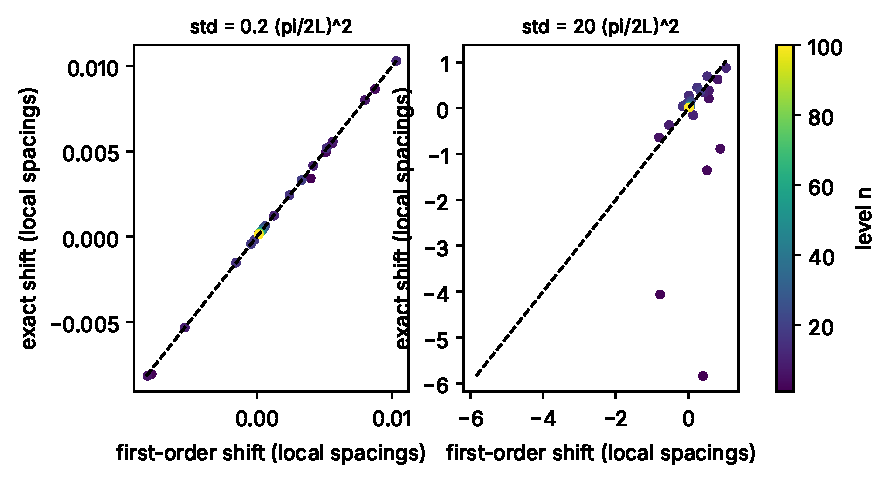
\includegraphics[width=0.95\linewidth]{figs/perturbation_scatter.pdf}
\caption{Exact level shifts versus first-order predictions for levels $n=1$--$100$ of the box $L=44.883$ perturbed by $\delta V=\sum_{k=0}^{19}c_k\cos(k\pi x/L)$ with random Gaussian coefficients, in units of the local spacing $(\pi/2L)^2\,2n$. Color encodes $n$. Left: coefficients of standard deviation $0.2(\pi/2L)^2$; the points lie on the diagonal. Right: standard deviation $20(\pi/2L)^2$; the first-order model fails, most strongly for the lowest levels, whose spacing is smallest.}
\label{fig:perturbation-scatter}
\end{figure}

\begin{pitfall}
\textbf{Truncated state sums.} In a computer, the second-order sum $\sum_{m\ne n}$ runs over a finite set of states. Terms from distant states are small, but terms from \emph{nearby} states are the largest of all. If level $n$ sits near the top of the states you kept, its nearest neighbours above are missing, and the truncated sum is badly biased. A drastic example is Problem~14: keeping only two states changes the second-order shift of box level 2 under a tilt from $+0.0052F^2$ to $+0.0175F^2$. The paper meets exactly this issue, \cref{sec:perturbation-paper}.
\end{pitfall}

\begin{keyideas}
\item Exact levels come from diagonalizing $H_{km}=E_k^{(0)}\delta_{km}+\delta V_{km}$ in a truncated basis, \cref{eq:perturbation-galerkin}, checking convergence in $N_b$.
\item Perturbation theory is reliable when couplings (and diagonal shifts) are small compared with the spacings of the coupled levels, \cref{eq:perturbation-validity}; this is a heuristic rule.
\item Spacings decide fragility: in the box low levels are fragile, in a potential with shrinking spacings high levels are.
\item Truncated state sums bias levels near the top of the kept set.
\end{keyideas}

%======================================================================
\section{Fitting by iterated linearization}\label{sec:perturbation-fitting}

\subsection{Turning the question around}

So far we asked: given $\delta V$, how do the levels move? A fit asks the reverse: given target values $\tilde t_n$ for the levels, which coefficients $\bm c$ make $E_n(\bm c)=\tilde t_n$? The relation between $\bm c$ and the levels is nonlinear, so we cannot solve it in one step. But we know its exact derivative, the sensitivity matrix \cref{eq:perturbation-HF}. That is precisely what Newton's method needs.

\subsection{One parameter: Newton's method}

Recall from Chapter~\ref{ch:asymptotics} that Newton's method solves $f(c)=0$ by replacing $f$ with its tangent line at the current guess $c_j$ and jumping to where the tangent crosses zero: $c_{j+1}=c_j-f(c_j)/f'(c_j)$. To make level $n$ equal a target $\tilde t$, take $f(c)=E_n(c)-\tilde t$; its derivative is $A_{nk}(c)$ by \cref{eq:perturbation-HF}. Writing the residual $r=\tilde t-E_n(c_j)$,
\begin{equation}
c_{j+1}=c_j+\frac{r}{A_{nk}(c_j)} .
\label{eq:perturbation-newton1}
\end{equation}

\begin{sample}{Fitting one level with one cosine}
Box with $L=1$, $\delta V=c\cos(\pi x/L)$. Find $c$ such that the ground state has energy $\tilde t=3$, by Newton's method starting at $c=0$.

\textbf{Step 1: First step.} At $c=0$: $E_1=\pi^2/4=2.467401$ and $A_{11}=+\tfrac12$ (\cref{eq:perturbation-boxcos}). The residual is $r=3-2.467401=0.532599$, so $c_1=0+0.532599/0.5=1.065198$. This is pure first-order perturbation theory: it would hit the target exactly if the levels were linear in $c$.

\textbf{Step 2: Evaluate exactly.} Exact diagonalization at $c_1$ gives $E_1(c_1)=2.985239$, short of the target by $r=0.014761$, because the second-order shift (always downward for the ground state) was ignored.

\textbf{Step 3: Recompute the sensitivity.} With the \emph{new} ground-state wavefunction, $A_{11}(c_1)=\int|\psi_1(c_1)|^2\cos(\pi x/L)\dd x=0.4719$. It is smaller than $\tfrac12$ because the perturbation has mixed some of level 3 into the ground state.

\textbf{Step 4: Second step.} $c_2=1.065198+0.014761/0.4719=1.0965$.

\textbf{Step 5: Check.} At $c_2$, the exact ground-state energy is $3.0000$ to four decimal places.

\[
\boxed{c\approx1.0965\ \text{after two Newton steps; }E_1=3.0000.}
\]
\Cref{fig:perturbation-newton} shows the two tangent lines. The first step overshoots in $c$ by about 3\%, the second step is already within $10^{-4}$ in energy: the quadratic convergence of Newton's method from Chapter~\ref{ch:asymptotics}.
\end{sample}

\begin{figure}[htbp]\centering
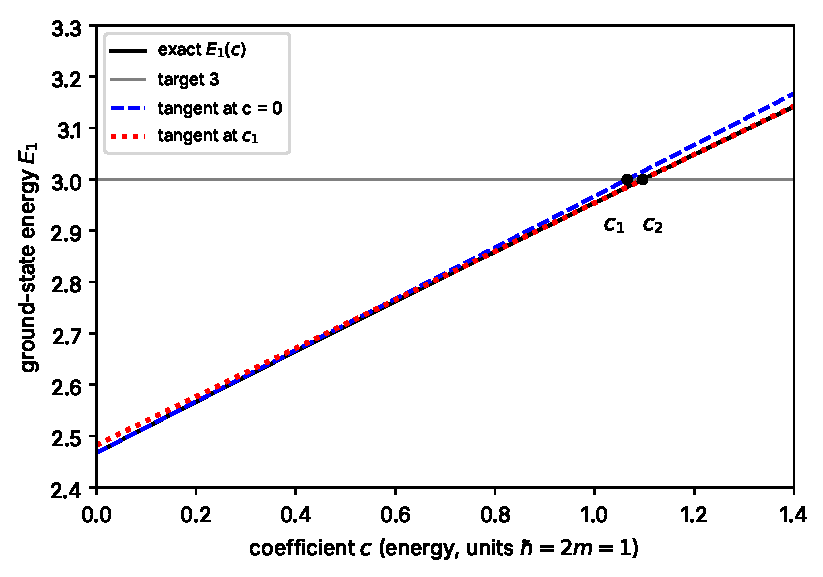
\includegraphics[width=0.85\linewidth]{figs/perturbation_newton.pdf}
\caption{Newton's method for fitting one level. Solid: the exact ground-state energy $E_1(c)$ of the box ($L=1$) with $\delta V=c\cos(\pi x/L)$. Horizontal line: the target $3$. Dashed: the tangent at $c=0$, whose slope is the first-order sensitivity $A_{11}=1/2$; it crosses the target at $c_1=1.0652$. Dotted: the tangent at $c_1$, slope $A_{11}(c_1)=0.4719$, crossing the target at $c_2=1.0965$, where $E_1$ already equals 3 to four decimals.}
\label{fig:perturbation-newton}
\end{figure}

\begin{pycode}
import numpy as np
L, Nb = 1.0, 60
n = np.arange(1, Nb + 1)
E0 = (n * np.pi / (2 * L))**2
D = np.abs(n[:, None] - n[None, :]); S = n[:, None] + n[None, :]
C1 = -0.5 * ((D == 2) * 1.0 - (S == 2) * 1.0)   # <n|cos(pi x/L)|m>

def ground(c):
    w, v = np.linalg.eigh(np.diag(E0) + c * C1)
    return w[0], v[:, 0] @ C1 @ v[:, 0]         # E_1 and dE_1/dc

c, target = 0.0, 3.0
for step in range(4):
    E1, A11 = ground(c)
    print(step, c, E1, A11)
    c = c + (target - E1) / A11                  # Newton update
\end{pycode}

The derivative in the listing, $v^{\top}C_1v$, is \cref{eq:perturbation-Ank} written in the basis of box states: if $\psi_1=\sum_ma_m\psi_m^{(0)}$ then $\int|\psi_1|^2\cos(\pi x/L)\dd x=\sum_{m,l}a_ma_l\bra{m}\cos\tfrac{\pi x}{L}\ket{l}$.

\subsection{Many parameters: the Gauss--Newton idea}

With many levels and many coefficients the same idea becomes a loop:
\begin{enumerate}
\item At the current $\bm c$, solve the eigenvalue problem of $H(\bm c)$ \emph{exactly} (numerically): levels $E_n(\bm c)$ and states $\psi_n(\bm c)$.
\item Form the residuals $r_n=\tilde t_n-E_n(\bm c)$.
\item Form the sensitivity matrix $A_{nk}(\bm c)=\int|\psi_n(\bm c)|^2\phi_k\,\dd x$.
\item Find a step $\Delta\bm c$ that makes the \emph{linearized} levels hit the targets: $\sum_kA_{nk}\Delta c_k\approx r_n$.
\item Set $\bm c\leftarrow\bm c+\Delta\bm c$ and return to step 1.
\end{enumerate}
If the number of target levels equals the number of coefficients and $A$ is invertible, step 4 is a square linear system (Chapter~\ref{ch:linear-algebra}), and the loop is Newton's method in many dimensions. In practice there are more levels than coefficients, or fewer, and step 4 becomes a least-squares problem (Chapter~\ref{ch:least-squares}); with that change the loop is called the Gauss--Newton method. When a full step is too bold (the linearization fails over the step's length), one shortens or damps it; Chapter~\ref{ch:fitting} develops this into the Levenberg--Marquardt method that the paper uses.

\begin{checkpoint}
Why recompute $A$ at every iteration instead of using the $A$ of the unperturbed potential throughout?
\end{checkpoint}
\checkanswer{Because $A_{nk}(\bm c)$ is the exact derivative only at the current $\bm c$. As $\bm c$ grows the wavefunctions change (in the sample, $A_{11}$ dropped from $0.5$ to $0.4719$), and using stale derivatives makes the steps aim at the wrong place; with the current $A$ the method converges quadratically near the solution.}

\subsection{Why this works, and what it does not need}

Notice what the loop asks of perturbation theory. It does \emph{not} require the final $\delta V$ to be small compared with level spacings. Each step only needs the linearization to be good over the length of that \emph{step}, and step 1 evaluates the levels exactly, so an inaccurate step is detected immediately and can be rejected or shortened. Perturbation theory is used as a \emph{step proposer}, never as the \emph{model}. The final coefficients can describe a correction far outside the perturbative regime of \cref{eq:perturbation-validity}, and the levels reported are still the true eigenvalues of the fitted operator.

The opposite strategy is to write the levels \emph{as} the perturbative formula, for example $E_n\approx E_n^{(0)}+\sum_kA_{nk}c_k+(\text{second-order terms})$, and to optimize that formula directly. This is cheaper (no eigensolve per step), but nothing stops the optimizer from choosing coefficients for which the formula no longer describes any operator. The formula then reports fits that the actual operator does not achieve. Sec.~V of the paper is an example, discussed next.

\begin{keyideas}
\item Fitting reverses perturbation theory: choose $\bm c$ to hit target levels.
\item The sensitivity matrix is the exact Jacobian, so Newton (one level) and Gauss--Newton (many levels) iterations use it directly.
\item Iterated linearization with exact eigensolves needs perturbation theory to hold only for each step; optimizing a perturbative formula as the model needs it to hold everywhere the optimizer goes.
\end{keyideas}

%======================================================================
\section{Paper connection}\label{sec:perturbation-paper}

\paragraph{The sensitivity matrix of Sec.~II~C.}
The paper's Hermitian fit perturbs the Wu--Sprung potential, $V\to V+\delta V$ with $\delta V(x)=\sum_{k=0}^{M-1}c_k\cos(k\pi x/L)$, and fits the coefficients ``by iterated linearization: solve for $(E_n,\psi_n)$; form residuals $r_n=\tilde t_n-E_n$ and the first-order sensitivity $A_{nk}=\int|\psi_n|^2\cos(k\pi x/L)\,dx$; update $c$ by SVD-damped least squares with a Levenberg--Marquardt schedule, accepting only steps that improve the rms'' (Sec.~II~C). Every ingredient is in this chapter: $A_{nk}$ is \cref{eq:perturbation-Ank}; evaluated with the current eigenfunctions it is the exact Jacobian, \cref{eq:perturbation-HF}; and the loop is the one of \cref{sec:perturbation-fitting}, with step 4 solved by damped least squares (App.~A, step 6, explained line by line in Chapter~\ref{ch:fitting}). The targets $\tilde t_n$ are the Riemann zeros corrected for the grid bias of the finite-difference solver, a correction explained in Chapter~\ref{ch:finite-differences}. App.~A, step 4, records that the eigenpairs come from \texttt{eigh\_tridiagonal}, so the normalization pitfall of \cref{sec:perturbation-sensitivity} applies.

\paragraph{Exact spectrum at every step.}
Because each iteration begins with an exact eigensolve and accepts only improving steps, the Hermitian fit uses perturbation theory as a step proposer only. This matters, because the fitted corrections are not small. In the interpolation split of Sec.~III, the fitted correction has ``rms $\delta V=40$'' in the band of turning points of the held-out levels and ``a maximum $|\delta V|=199$ where the smooth potential is about $500$'' (Sec.~III, Fig.~4). For comparison, near levels 201--300 the mean spacing of the zeros is about 1.46 (it is the quantity $\mathrm{gap}_n=2\pi/\log(s_n/2\pi)$ of Sec.~II~A, studied in Chapter~\ref{ch:counting-zeros}). A single linearization from $\bm c=0$ would be useless at that size (our estimate from \cref{eq:perturbation-validity}, not a statement of the paper); the paper's in-sample and out-of-sample numbers are nonetheless the true eigenvalues of the fitted operators, scored by ``a single plain eigensolve of the fitted potential'' (Sec.~II~C).

\paragraph{A level probes the potential near its turning points.}
The first-order formula says a level responds to $\delta V$ where $|\psi_n|^2$ is large, and \cref{sec:perturbation-first} noted that for high levels the density is largest near the classical turning points. The paper uses this in Sec.~III: ``Position maps to level index through the classical turning point, and levels 201--300 turn at $x=22.5$--$28.5$,'' which is exactly where the unregularized fit placed its largest structure. Chapter~\ref{ch:wkb} makes the turning-point picture quantitative.

\paragraph{The coverage law.}
Sec.~III reports that the fit reaches rms $0.186$ on all 500 zeros at $M=300$ and below $10^{-4}$ spacings by $M=900$, ``consistent with a basis-coverage law (the cosine family becomes effectively complete for joint level shifts once $M\pi/L>2\sqrt E$)''. The box gives an exact miniature of this law. In the box $2\sqrt{E_n}=n\pi/L$, so $M\pi/L>2\sqrt{E_n}$ means $M>n$: by \cref{eq:perturbation-Abox}, level $n$ can be moved independently only if the cosine with $k=n$ is in the basis. Reading the condition as $E<(M\pi/2L)^2$ with $L=44.883$ gives $E<110$ for $M=300$, $E<196$ for $M=400$, and $E<992$ for $M=900$; the 500th zero is at $t_{500}=811.18$ (App.~A, key anchors), inside the last range only. This is consistent with the paper's numbers, but remember the paper calls it a law with which the results are ``consistent'', and Chapter~\ref{ch:fitting} derives it only heuristically. \Cref{fig:perturbation-sensitivity} also shows why the Wu--Sprung problem is less tidy than the box: low cosines act almost like the constant mode for low levels, so several columns of $A$ are nearly alike, the kind of near-redundancy that makes a linear system ill-conditioned (Chapter~\ref{ch:least-squares}).

\paragraph{The second-order formula of Eq.~(5).}
Sec.~II~E perturbs $H\to H+iA$, where $A=\sum_kc_k\phi_k$ is a real function and $i$ is the imaginary unit. Our general results \cref{eq:perturbation-first,eq:perturbation-second-general} needed only $H_0$ to be Hermitian, so they apply with $W=iA$. First order gives $iA_{nn}$, purely imaginary, so the leading \emph{real} shift is second order:
\[
\sum_{m\ne n}\frac{(iA)_{nm}(iA)_{mn}}{E_n-E_m}=i^2\sum_{m\ne n}\frac{A_{nm}A_{mn}}{E_n-E_m}=-\sum_{m\ne n}\frac{|A_{nm}|^2}{E_n-E_m},
\]
which is the paper's Eq.~(5); the sign is opposite to the Hermitian \cref{eq:perturbation-second} because $i^2=-1$. Since $A_{nm}=\sum_kc_k(\phi_k)_{nm}$ with $(\phi_k)_{nm}=\bra{n}\phi_k\ket{m}$, the shift is a quadratic form in $\bm c$: $-\bm c^{\top}T^{(n)}\bm c$ with $T^{(n)}_{kl}=\sum_{m\ne n}(\phi_k)_{nm}(\phi_l)_{nm}/(E_n-E_m)$. Chapter~\ref{ch:non-hermitian} works all of this out carefully, including decay and PT symmetry. Two details already make sense here. (a) The PT-odd class uses $\phi_k=\sin((k+1)\pi x/L)$, odd functions, and the paper notes ``$A_{nn}=0$'': this is the parity argument of \cref{sec:perturbation-first}, exactly as for our tilt. (b) The state sum runs ``over all 652 basis states with $E\le1000$ (truncating at 500 states measurably biases the top levels)'': this is the truncation pitfall of \cref{sec:perturbation-validity}.

\paragraph{Sec.~V: leaving the perturbative regime.}
In Sec.~V the second-order formula is not a step proposer: it is the model that the optimizer minimizes (the ``surrogate''). The paper then checks it against exact diagonalization of $H+iA$, as recommended in \cref{sec:perturbation-fitting}. At the fitted amplitude, ``corr(exact, second-order) drops to $+0.14$/$+0.18$ (odd/even), the surrogate overstates shift magnitudes twofold (Fig.~5, left), and 3\% of eigenstates can no longer be matched one-to-one to unperturbed states.'' Scoring the exact spectra in-sample gives rms $0.2523$ and $0.2477$, worse than the null $0.2438$. ``At quarter amplitude the surrogate is accurate (corr $+0.88$/$+0.94$)'', and amplitude-controlled fits with $\lVert c\rVert\le R$, $R=4$, ``pass exact verification (corr $+0.93$/$+0.995$, all states matched)''. This is \cref{fig:perturbation-scatter} at full scale: small amplitude, agreement; large amplitude, the formula describes no operator. Hence the paper's standard (ii) in Sec.~VI: ``scoring of the actual operator spectrum, not a surrogate.''

\paragraph{The constant mode.}
Sample Problem ``A constant shift'' showed that $\phi_0=1$ shifts every level equally and couples no states. For $H+iA$ a constant therefore shifts all levels by the same imaginary constant and has zero second-order real shift (Sec.~II~E, safeguard (i)); its tensor rows are exactly zero. Sec.~V reports that before this was enforced, the optimizer ``had driven the exactly-null constant mode to $c_0\approx2.2\times10^{6}$, harvesting in-sample improvement from float32 noise''. Chapter~\ref{ch:paper-spurious-floor} dissects the episode.

\paragraph{A warning about the symbol $A$.}
The paper uses $A$ for two different things: the sensitivity matrix $A_{nk}$ of Sec.~II~C and the non-Hermitian operator $A$ of Sec.~II~E, whose matrix elements are $A_{nm}=\bra{n}A\ket{m}$. They are related (both are integrals of products of wavefunctions and basis functions) but not the same object. In this chapter $A_{nk}$ always means the sensitivity matrix.

\paragraph{Memorization, previewed.}
Sample Problem ``Tuning three box levels'' fitted three targets exactly while predicting nothing about level 4 beyond a common offset. The paper's central negative result (Sec.~III, Table~I) is a far richer version of this phenomenon, analysed in Chapters~\ref{ch:generalization} and~\ref{ch:paper-memorization}; do not read the toy as an explanation of it, only as a first picture.

%======================================================================
\section{Summary}\label{sec:perturbation-summary}

\begin{itemize}
\item Write $H=H_0+\delta V$, $\delta V=\varepsilon W$, and expand energies and states in powers of $\varepsilon$ (assumption justified for nondegenerate levels; \cref{sec:perturbation-tools}). Matrix elements: $W_{nm}=\int\psi_n^{(0)*}W\psi_m^{(0)}\dd x$, \cref{eq:perturbation-matel}.
\item First order: $\delta E_n^{(1)}=\delta V_{nn}=\int|\psi_n^{(0)}|^2\delta V\,\dd x$, \cref{eq:perturbation-first}: a density-weighted average.
\item Constant $\delta V$: exact uniform shift. Odd $\delta V$ in an even potential: zero first-order shift. Box with cosines: $\cos(q\pi x/L)$ moves only level $q$, by $(-1)^{q+1}c/2$, \cref{eq:perturbation-boxcos}.
\item For $\delta V=\sum_kc_k\phi_k$: $\delta\bm E\approx A\bm c$, $A_{nk}=\int|\psi_n|^2\phi_k\dd x$, \cref{eq:perturbation-linear,eq:perturbation-Ank}; with current states $A_{nk}=\partial E_n/\partial c_k$ exactly, \cref{eq:perturbation-HF}.
\item First-order state: \cref{eq:perturbation-psi1}. Second order: $\sum_{m\ne n}\delta V_{nm}\delta V_{mn}/(E_n^{(0)}-E_m^{(0)})$, equal to $\sum_{m\ne n}|\delta V_{nm}|^2/(E_n^{(0)}-E_m^{(0)})$ for real $\delta V$, \cref{eq:perturbation-second-general,eq:perturbation-second}.
\item Level repulsion: levels above push down, below push up; exact two-level formula \cref{eq:perturbation-twolevel}; avoided crossings.
\item Box matrix elements: $x_{nm}$, \cref{eq:perturbation-xnm}; cosines, \cref{eq:perturbation-cosmat}.
\item Exact levels from the matrix \cref{eq:perturbation-galerkin} in a truncated basis.
\item Validity (heuristic): couplings and shifts small compared with spacings of coupled levels, \cref{eq:perturbation-validity}.
\item Fitting: Newton, \cref{eq:perturbation-newton1}, and Gauss--Newton loops using $A$ as the Jacobian with exact eigensolves; optimizing a perturbative formula itself is safe only inside its validity range (paper Sec.~V).
\end{itemize}

%======================================================================
\section{Problems}\label{sec:perturbation-problems}

\begin{problemlist}
\prob{1}{A box with $L=2$ has its potential raised by the constant $\delta V=0.3$. Find the first-order and second-order shifts of level 5, and the exact shift.}

\prob{1}{In the symmetric box, $\delta V=Fx^3$. Without computing any integral, find the first-order shift of every level.}

\prob{1}{Show that for any normalized state the sensitivity to the constant basis function $\phi_0=1$ is $A_{n0}=1$. What does the column of ones mean physically?}

\prob{1}{Box with $L=1$ and $\delta V=c\cos(2\pi x/L)$. Find the first-order shifts of levels 1, 2 and 3.}

\prob{1}{A two-level system has $E_1=0$, $E_2=2$ and coupling $v=0.1$. Find the second-order estimates of both levels and the exact eigenvalues.}

\prob{2}{Prove that the second-order shift of the ground state is never positive. For a finite $N_b\times N_b$ matrix, what can you say about the sign of the second-order shift of the highest level?}

\prob{2}{Box with $\delta V=c\cos(\pi x/L)$. Show that level 2 has zero first-order shift and that its second-order shift is $-c^2L^2/(12\pi^2)$. Evaluate for $L=1$, $c=1$.}

\prob{2}{For the tilted box ($L=1$, $\delta V=Fx$), compute the second-order shift of level 2, summing the contributions of $m=1,3,5,7$. Explain its sign using level repulsion.}

\prob{2}{Derive the Hellmann--Feynman theorem directly: if $H(\lambda)\psi_n(\lambda)=E_n(\lambda)\psi_n(\lambda)$ with $\int|\psi_n|^2\dd x=1$ for all $\lambda$, show that $\dd E_n/\dd\lambda=\int\psi_n^*(\partial H/\partial\lambda)\psi_n\dd x$, using \cref{eq:perturbation-hermitian}.}

\prob{2}{For $\delta V=c\cos(\pi x/L)$ in the box, use \cref{eq:perturbation-validity} to show that the condition for level $n\ge3$ is $c\ll8(n-1)(\pi/2L)^2$ and that higher levels are more robust. Evaluate the $n=1$ condition for $L=1$.}

\prob{2}{(Paper.) In Table~I of the paper, the scale-1 fits on zeros 1--400 use $M=200$, $400$ and $600$, and a scale-2 fit on zeros 1--800 uses $M=900$. Give the dimensions of the sensitivity matrix $A_{nk}$ restricted to the training levels in each case, and say which linearized systems have more unknowns than equations.}

\prob{2}{(Paper.) In the paper's interpolation split (Sec.~III, Fig.~4), the fitted correction has rms 40 in the turning-point band of levels 201--300, while the mean spacing there is about 1.46. Is a single first-order linearization from $\bm c=0$ adequate to describe this fitted potential? Why are the paper's predicted levels nonetheless trustworthy as eigenvalues of the fitted operator?}

\prob{2}{(Paper.) Sec.~V of the paper reports that at the fitted amplitude the correlation between exact and second-order shifts is only $+0.14$/$+0.18$, but at quarter amplitude it is $+0.88$/$+0.94$. Assuming the perturbation series converges, explain with a scaling argument why reducing all coefficients by a factor 4 should make the second-order formula more accurate.}

\prob{2}{(Paper.) Compute the second-order shift of box level 2 under a tilt ($L=1$) keeping only states 1 and 2 in the sum, and compare with your result of Problem~8. Use the comparison to explain the paper's remark (Sec.~II~E) that truncating the state sum at 500 states ``measurably biases the top levels'', and why it sums over all 652 states with $E\le1000$.}

\prob{2}{Using numpy and the matrix method of \cref{sec:perturbation-validity}, compute the error of the second-order formula for the box ground state with $\delta V=c\cos(\pi x/L)$, $L=1$, at $c=1$ and $c=0.5$. Show that the ratio of the errors is close to 8, and explain why.}

\prob{2}{Using qmnt (\texttt{qmnt.L\_of}, \texttt{qmnt.grid}, \texttt{qmnt.wu\_sprung\_V}, \texttt{qmnt.fd\_levels} with \texttt{return\_vectors=True}) or the listing of \cref{sec:perturbation-sensitivity}, compute $A_{nk}$ for the Wu--Sprung potential for $n\le50$ and $k\le50$ on a 2000-point grid. Verify that column $k=0$ equals 1, and reproduce the right panel of \cref{fig:perturbation-sensitivity} qualitatively. Then set the potential to zero and recover \cref{eq:perturbation-Abox} approximately.}

\prob{2}{For the two-level matrix $H(\lambda)=\begin{pmatrix}\lambda&v\\v&-\lambda\end{pmatrix}$, find the exact eigenvalues, the minimum gap, and the behavior for $|\lambda|\gg|v|$. Show that the latter agrees with second-order perturbation theory.}

\prob{2}{For $\delta V=c\cos(q\pi x/L)$ in the box, show that level $n=q$ (with $q\ge1$) couples only to level $3q$, and that its second-order shift is $-c^2L^2/(8\pi^2q^2)$.}

\prob{3}{\emph{Sum rule.} Let $W$ be real and consider a finite set of $N_b$ nondegenerate levels. Show that $\sum_{n=1}^{N_b}E_n^{(2)}=0$ (a) by pairing the $(n,m)$ and $(m,n)$ terms, and (b) by using the fact that the trace of the matrix $H_{km}$ equals the sum of its eigenvalues. (This sum rule reappears for $H+iA$ in Sec.~V~A of the paper.)}

\prob{3}{Using the Hellmann--Feynman theorem and the first-order wavefunction \cref{eq:perturbation-psi1}, show that for $H(\lambda)=H_0+\lambda W$ one has $\dd^2E_n/\dd\lambda^2\big|_{\lambda=0}=2E_n^{(2)}$.}

\prob{3}{For the tilted ground state of the $L=1$ box, use Hellmann--Feynman to show that the expectation value of position is $\langle x\rangle=\dd E_1/\dd F$, and evaluate it to first order in $F$. In which direction does the particle move, and why does that make physical sense?}

\prob{2}{Using numpy, sum the series $S=\sum_{m=2,4,6,\dots}m^2/(m^2-1)^5$ to $m=1000$ and check that it agrees with $(15-\pi^2)\pi^2/3072$.}

\prob{2}{(Paper.) App.~A of the paper uses $L=44.8827$ and a working grid of $N=6000$ interior points at scale 1. Compute the grid spacing $h=2L/(N+1)$. If you forgot to divide the eigenvectors from \texttt{eigh\_tridiagonal} by $\sqrt h$, by what factor would every $A_{nk}$ be wrong, and what would that do to an undamped Gauss--Newton step?}

\prob{3}{(Paper.) Contrast the role of perturbation theory in the paper's Hermitian fit (Sec.~II~C, App.~A step 6) with its role in the non-Hermitian fit (Sec.~II~E, App.~A step 10). Explain why the first is protected against the failure documented in Sec.~V and the second is not, and how the safeguards (ii) and (iii) of Sec.~II~E repair the second.}

\prob{2}{Using numpy and the Newton listing of \cref{sec:perturbation-fitting}, fit the box ground state ($L=1$, $\delta V=c\cos(\pi x/L)$) to the target $3.5$. Give the first Newton iterate by hand, and count the iterations needed until $|E_1-3.5|<10^{-10}$.}
\end{problemlist}

%======================================================================
\section{Answers to selected problems}\label{sec:perturbation-answers}

\textbf{1.} First order: $\int|\psi_5^{(0)}|^2(0.3)\dd x=0.3$. Second order: the off-diagonal elements $0.3\int\psi_5^{(0)}\psi_m^{(0)}\dd x=0.3\,\delta_{5m}$ vanish, so the shift is 0. Exact: $H_0+0.3$ has the same eigenfunctions with every energy raised by $0.3$ (as in the first Sample Problem), so the exact shift is $0.3$.

\textbf{2.} All zero. In the symmetric box every $|\psi_n^{(0)}|^2$ is even and $x^3$ is odd, so the integrand of \cref{eq:perturbation-first} is odd and integrates to zero over $[-L,L]$.

\textbf{3.} $A_{n0}=\int|\psi_n|^2\cdot1\,\dd x=1$ by normalization. Physically, raising the potential by the constant $c_0$ raises every level by $c_0$ at first order (exactly, in fact), whatever the state.

\textbf{4.} By \cref{eq:perturbation-boxcos} with $q=2$: only $n=2$ shifts, by $(-1)^{3}c/2=-c/2$. Levels 1 and 3: 0.

\textbf{5.} Second order: $\mp|v|^2/(E_2-E_1)=\mp0.01/2$, so $-0.005$ and $2.005$. Exact: $\Delta=1$, $\lambda_\pm=1\pm\sqrt{1.01}=1\pm1.0049876$, that is $-0.0049876$ and $2.0049876$. The agreement is good because $|v|/\Delta=0.1$.

\textbf{7.} With $q=1$, \cref{eq:perturbation-cosmat} gives a diagonal element only for $n=1$, so level 2 has none. Level 2 couples to $m$ with $|2-m|=2$, i.e.\ $m=4$ ($m=0$ does not exist), and $2+m=2$ is impossible for $m\ge1$. $\delta V_{24}=-c/2$, and $E_2^{(0)}-E_4^{(0)}=(\pi/2L)^2(4-16)=-3\pi^2/L^2$. The shift is $(c^2/4)/(-3\pi^2/L^2)=-c^2L^2/(12\pi^2)$, which for $L=c=1$ is $-0.0084434$.

\textbf{9.} Differentiate $E_n=\int\psi_n^*H\psi_n\dd x$ with the product rule: $\dd E_n/\dd\lambda=\int\psi_n^{*\prime}H\psi_n+\int\psi_n^*H'\psi_n+\int\psi_n^*H\psi_n'$, primes denoting $\partial/\partial\lambda$. The first term is $E_n\int\psi_n^{*\prime}\psi_n$. In the third use \cref{eq:perturbation-hermitian}: $\int\psi_n^*H\psi_n'=\int(H\psi_n)^*\psi_n'=E_n\int\psi_n^*\psi_n'$ ($E_n$ real). Together the first and third give $E_n\,\dd/\dd\lambda\int|\psi_n|^2\dd x=E_n\cdot0$, since the normalization is constant. What remains is $\int\psi_n^*H'\psi_n\dd x$.

\textbf{11.} Rows are levels, columns are basis functions. Scale 1, fit 1--400: $400\times200$ (more equations than unknowns), $400\times400$ (square), $400\times600$ (more unknowns than equations). Scale 2, fit 1--800, $M=900$: $800\times900$ (more unknowns than equations). For the last two the linearized step has infinitely many solutions unless something (damping, regularization, the minimum-norm choice of Chapter~\ref{ch:least-squares}) selects one.

\textbf{13.} If the series converges, the error of stopping after second order is dominated by the third-order term, which contains three factors of the perturbation and so scales as $c^3$, while the second-order term scales as $c^2$. The relative erroris roughly the ratio of the two, $c^3/c^2=c$, so it falls in proportion to the amplitude. Reducing every coefficient by a factor 4 multiplies the second-order shift by $1/16$ and the leading neglected term by $1/64$, so the neglected part shrinks four times faster than the part kept. In terms of \cref{eq:perturbation-validity}, the ratios $|\delta V_{nm}|/|E_n-E_m|$ all fall by 4, moving the fit back toward the perturbative regime. That is why the paper's quarter-amplitude check, corr $+0.88$/$+0.94$ (Sec.~V), succeeds where the full amplitude fails. If the series does not converge (or converges very slowly) at the fitted amplitude, the argument says nothing there. This is part of the reason exact diagonalization is the only safe judge.

\textbf{15.} With $N_b=60$: at $c=1$ the error of the second-order value is $2.954736-2.954413=3.2\times10^{-4}$. At $c=0.5$ the error is close to one eighth of that. The ratio is close to $2^3=8$ because the leading neglected term is third order (it contains, for example, the product $\delta V_{11}|\delta V_{13}|^2$), which scales as $c^3$. Halving $c$ divides it by 8.

\textbf{17.} $\det(H-\mu I)=(\lambda-\mu)(-\lambda-\mu)-v^2=\mu^2-\lambda^2-v^2=0$, so the eigenvalues are $\mu_\pm=\pm\sqrt{\lambda^2+v^2}$. The gap $2\sqrt{\lambda^2+v^2}$ is smallest at $\lambda=0$, where it equals $2|v|$. For $|\lambda|\gg|v|$ use $\sqrt{1+y}\approx1+y/2$ with $y=v^2/\lambda^2$: $\mu_\pm\approx\pm\bigl(|\lambda|+v^2/(2|\lambda|)\bigr)$. Perturbatively, level $\lambda$ couples to level $-\lambda$ with denominator $\lambda-(-\lambda)=2\lambda$, so its shift is $v^2/(2\lambda)$. For $\lambda>0$ this pushes the upper level up by $v^2/2|\lambda|$; the other level is pushed down by the same amount. This matches the expansion of the exact result.

\textbf{19.} (a) The second-order sum over all levels is $\sum_n\sum_{m\ne n}|W_{nm}|^2/(E_n^{(0)}-E_m^{(0)})$. Group the terms $(n,m)$ and $(m,n)$. They have the same numerator ($|W_{nm}|=|W_{mn}|$, by \cref{eq:perturbation-hermmat}) and opposite denominators, so each pair sums to zero. (b) The trace of $H_{km}=E_k^{(0)}\delta_{km}+\varepsilon W_{km}$ is $\sum_kE_k^{(0)}+\varepsilon\sum_kW_{kk}$ exactly, and the trace equals the sum of the eigenvalues (Chapter~\ref{ch:eigen}). Therefore $\sum_nE_n=\sum_nE_n^{(0)}+\varepsilon\sum_nW_{nn}$ holds for every $\varepsilon$. Comparing powers of $\varepsilon$, the sum over $n$ of every correction beyond first order vanishes, and in particular $\sum_nE_n^{(2)}=0$.

\textbf{21.} Here $\partial H/\partial F=x$, so Hellmann--Feynman, \cref{eq:perturbation-HF}, gives $\dd E_1/\dd F=\int|\psi_1|^2x\,\dd x=\langle x\rangle$. Through second order, $E_1\approx E_1^{(0)}-0.017556F^2$, so $\langle x\rangle\approx-0.035112F$. For $F>0$ the potential $Fx$ is lower on the left, and the particle shifts toward negative $x$. This is the direction of the force $-\dd(Fx)/\dd x=-F$.

\textbf{23.} The spacing is $h=2(44.8827)/6001=0.014958$. Without the division, every $A_{nk}$ is multiplied by $h$, so it is too small by the factor $1/h=66.85$. An undamped step solves $A\Delta\bm c=\bm r$, so $\Delta\bm c$ would be $66.85$ times too large. The linearization would fail badly over such a step. With the paper's accept-only-improvements rule, the step would be rejected and the damping would increase until the step shrank back, wasting iterations. Without that rule, the fit would diverge.

\textbf{25.} The first iterate is $c_1=(3.5-2.467401)/0.5=2.065198$. The Newton loop reaches $|E_1-3.5|<10^{-10}$ in fewer than six iterations. Each iteration roughly squares the error, the quadratic convergence of Chapter~\ref{ch:asymptotics}.
